\documentclass{beamer} 
\usepackage{amsmath,amsthm}
\usepackage{graphicx,microtype,parskip}
\usepackage{caption,subcaption,multirow}
\usepackage{attrib}

\frenchspacing

\usetheme{default}
\usecolortheme{whale}

\setbeamertemplate{navigation symbols}{}

\setbeamercolor{title}{fg=blue,bg=white}

\setbeamercolor{block title}{fg=white,bg=gray}
\setbeamercolor{block body}{fg=black,bg=lightgray}

\setbeamercolor{block title alerted}{fg=white,bg=darkgray}
\setbeamercolor{block body alerted}{fg=black,bg=lightgray}

%\AtBeginSection[]
%{
%  \begin{frame}
%    \tableofcontents[currentsection]
%  \end{frame}
%}


\title{Gambling with Australian brachiopods}
\author{Peter D Smits}
\institute{Committee on Evolutionary Biology, University of Chicago}

\begin{document}

\begin{frame}
  \maketitle
\end{frame}


\begin{frame}
  \frametitle{Gambler's Ruin}

  \begin{definition}
    Given infinite time, all gambler's go bust. 
  \end{definition}
\end{frame}


\begin{frame}
  \frametitle{Death of a taxon}

  \begin{block}{Taxa as gamblers}
    All taxa, given infinite time, go extinct.
  \end{block}
\end{frame}


\begin{frame}
  \frametitle{Foundation}

  \begin{alertblock}{Question}
    Why do taxa go extinct at \alert{different rates}?
  \end{alertblock}
\end{frame}


%\begin{frame}
%  \frametitle{Multi-level selection}
%  \begin{block}{Given a taxon level}
%    Impossible to determine if \alert{random} with respect to lower level without more information.
%  \end{block}
%\end{frame}

\begin{frame}
  \frametitle{Enter brachiopods}
  \begin{center}
    \noindent
    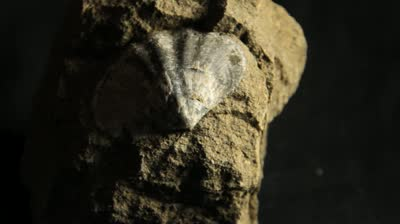
\includegraphics[height = 0.5\textheight, width = 0.4\textwidth, keepaspectratio = true]{figure/stock-brac1}\hspace{0.2\textwidth}%
    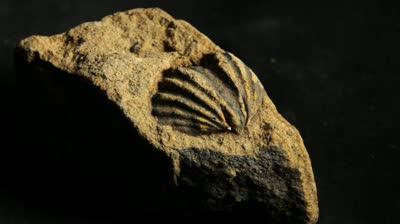
\includegraphics[height = 0.5\textheight, width = 0.4\textwidth, keepaspectratio = true]{figure/stock-brac2}\\[2em]
    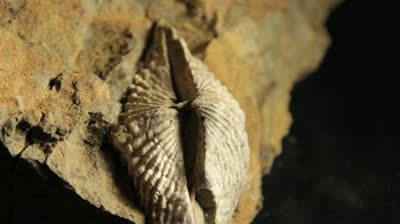
\includegraphics[height = 0.5\textheight, width = 0.4\textwidth, keepaspectratio = true]{figure/stock-brac3}\hspace{0.2\textwidth}%
    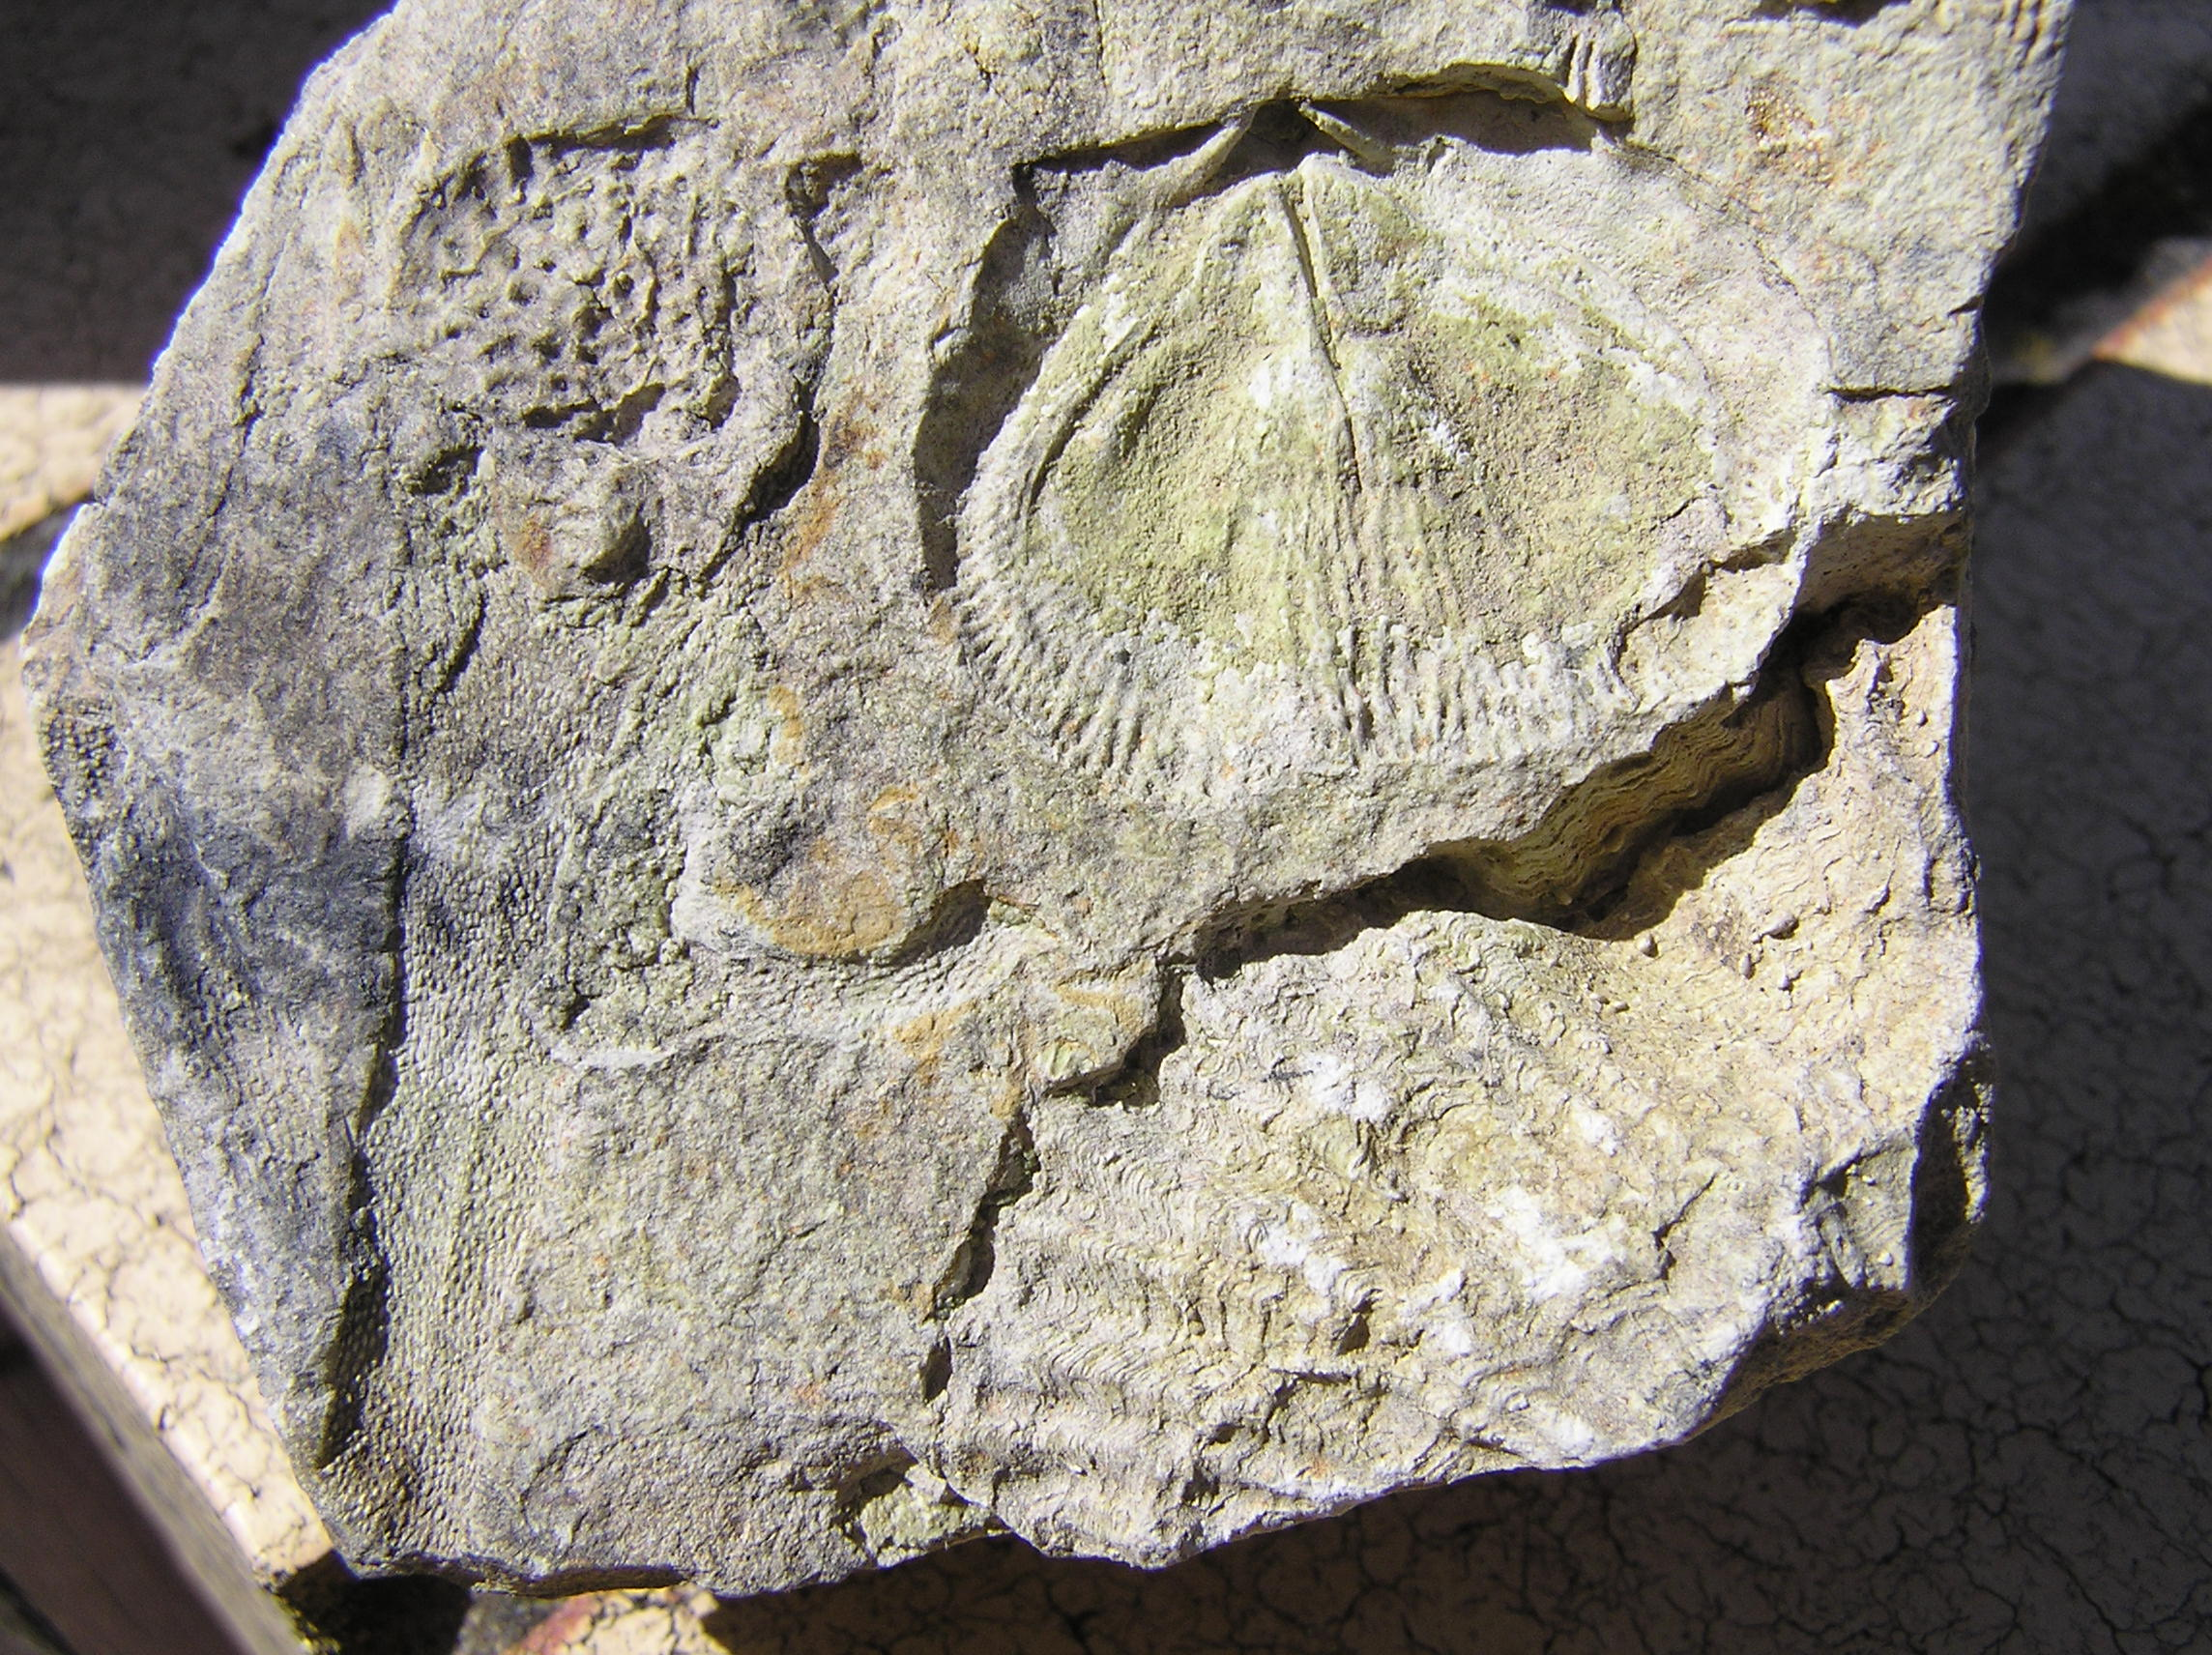
\includegraphics[height = 0.5\textheight, width = 0.4\textwidth, keepaspectratio = true]{figure/wiki_brac}\par

    \tiny{\attrib{Immersion Imagery, Shutterstock; Wikimedia}}
  \end{center}
\end{frame}

\begin{frame}
  \frametitle{System details}
  \begin{columns}
    \begin{column}{0.5\textwidth}
      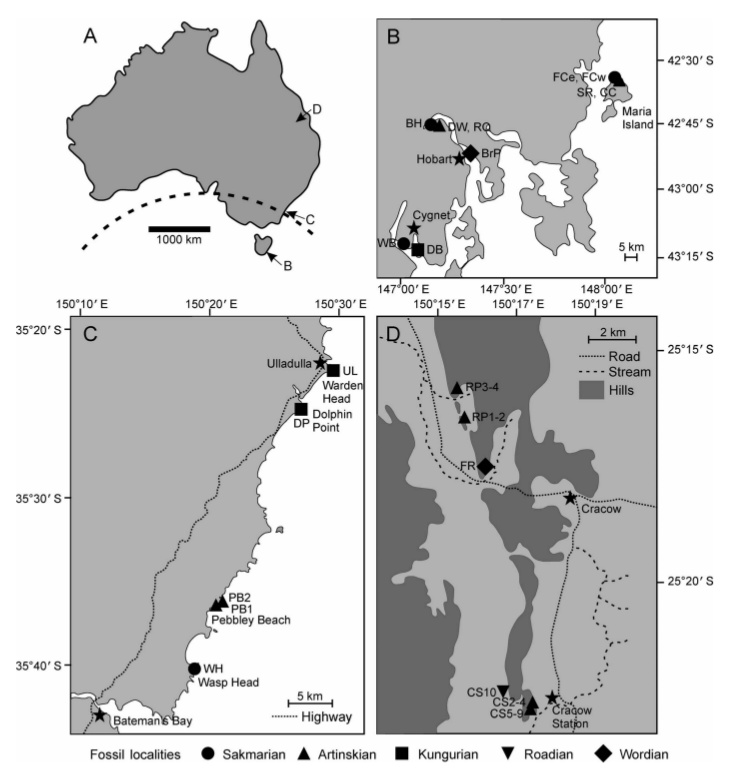
\includegraphics[height = 0.8\textheight, width = \textwidth, keepaspectratio = true]{figure/australia}

      \tiny{\attrib{Clapham and James 2008 \textit{Palaios}}}
    \end{column}
    \begin{column}{0.5\textwidth}
      \begin{itemize}
        \item Australian Permian
          \begin{itemize}
            \item range in/out taxa right censored
          \end{itemize}
        \item predictors 
          \begin{itemize}
            \item substrate probability (fully Bayesian approach)
            \item onshore/offshore
            \item body size (Payne \textit{et al.} 2014 \textit{Proc. B})
            \item occupancy (see Vilhena \textit{et al.} 2014 \textit{Nature Com.})
          \end{itemize}
      \end{itemize}
    \end{column}
  \end{columns}
\end{frame}


\begin{frame}
  \frametitle{Survival analysis}

  \begin{center}
    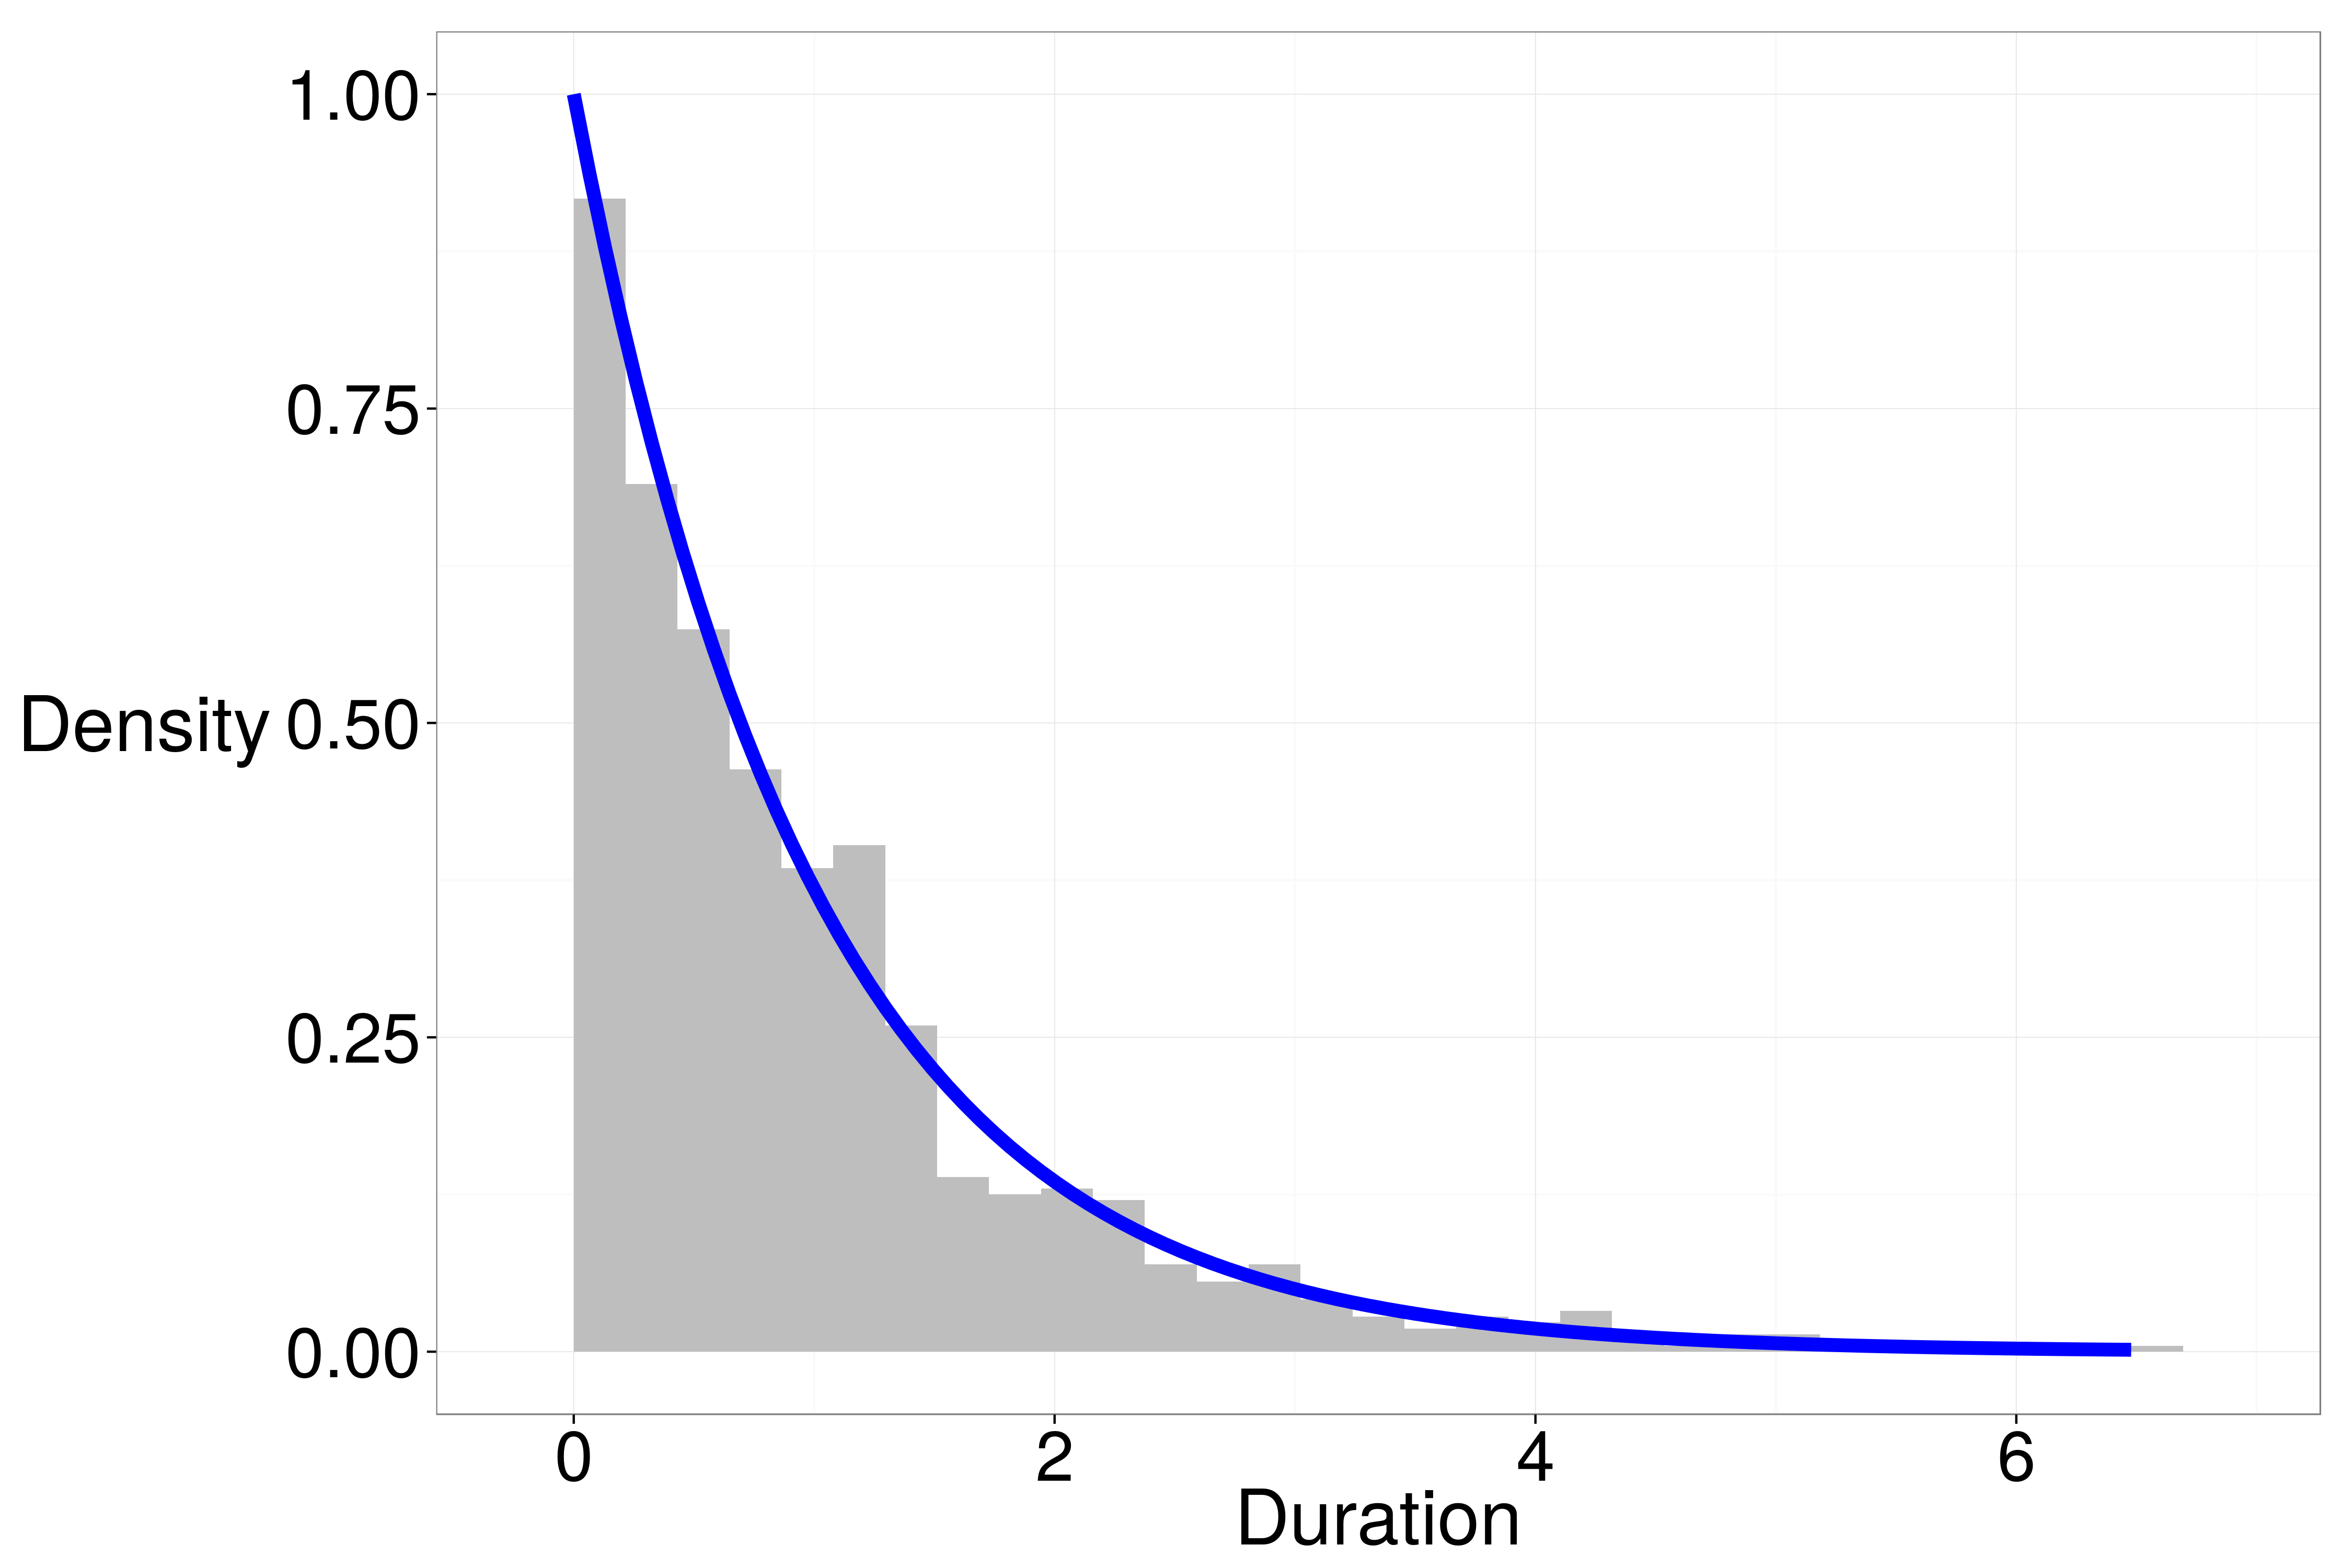
\includegraphics[height = 0.5\textheight, width = \textwidth, keepaspectratio = true]{figure/dur_exp}

    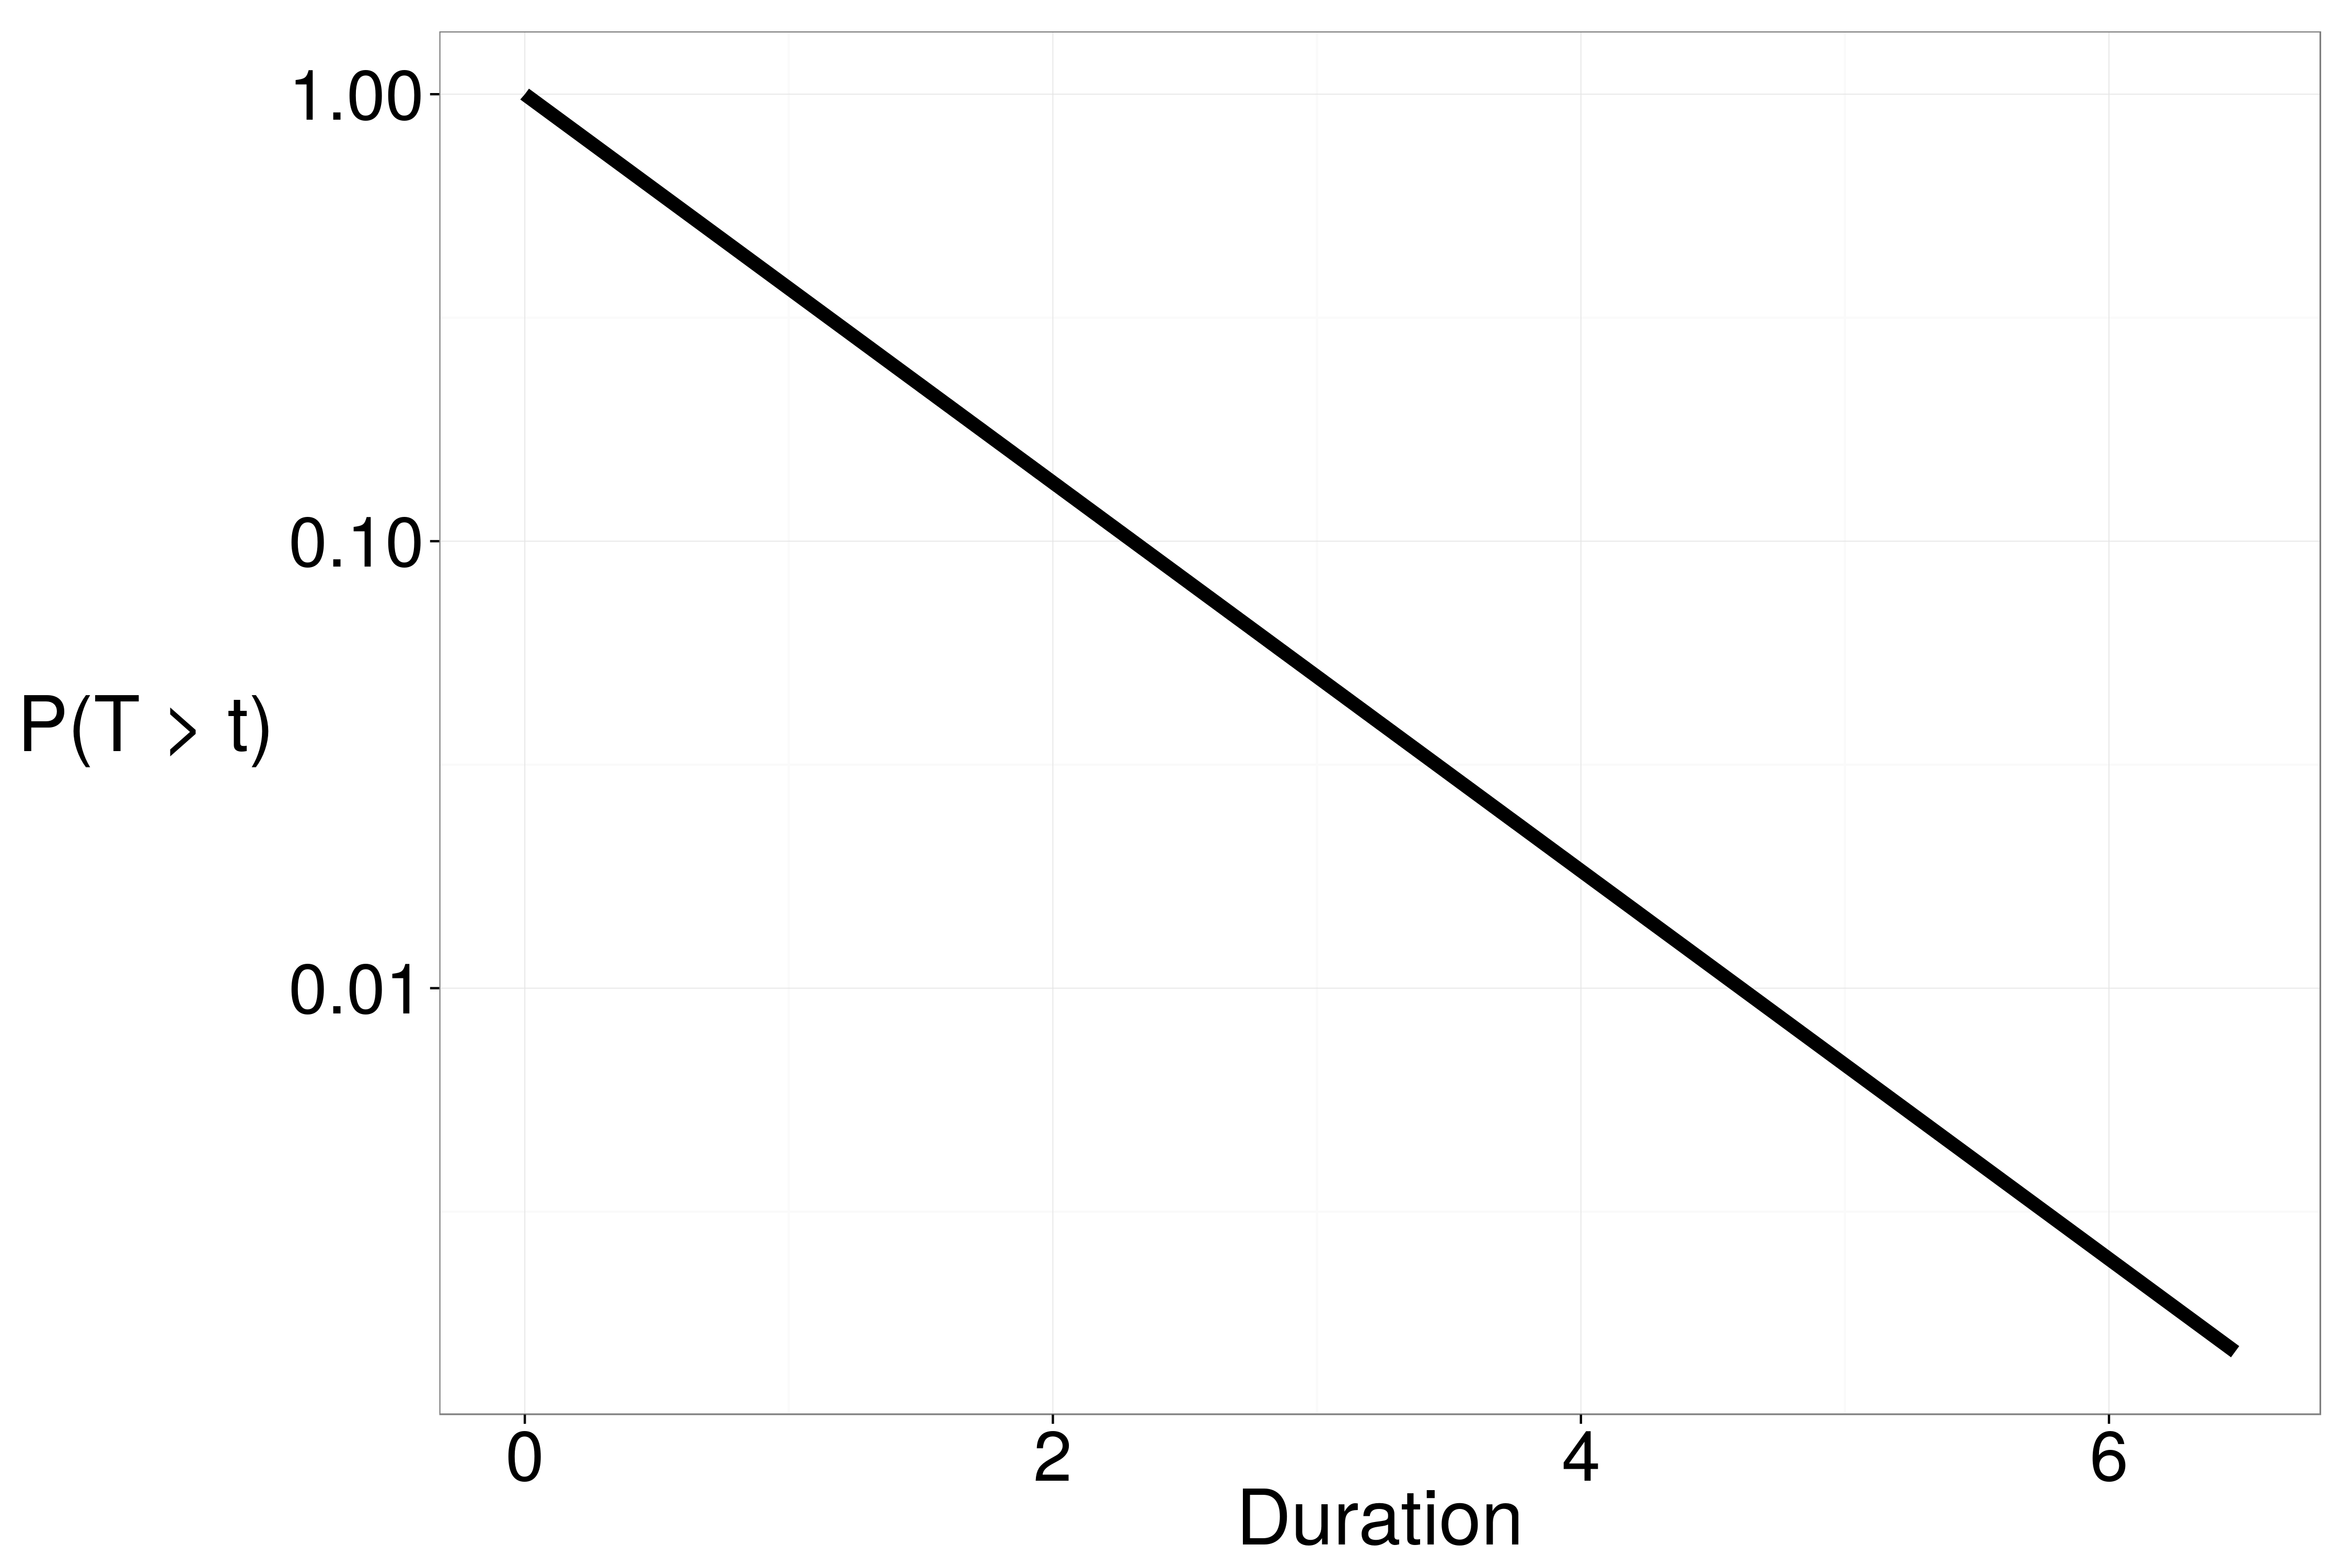
\includegraphics[height = 0.5\textheight, width = 0.4\textwidth, keepaspectratio = true]{figure/sur_exp}
    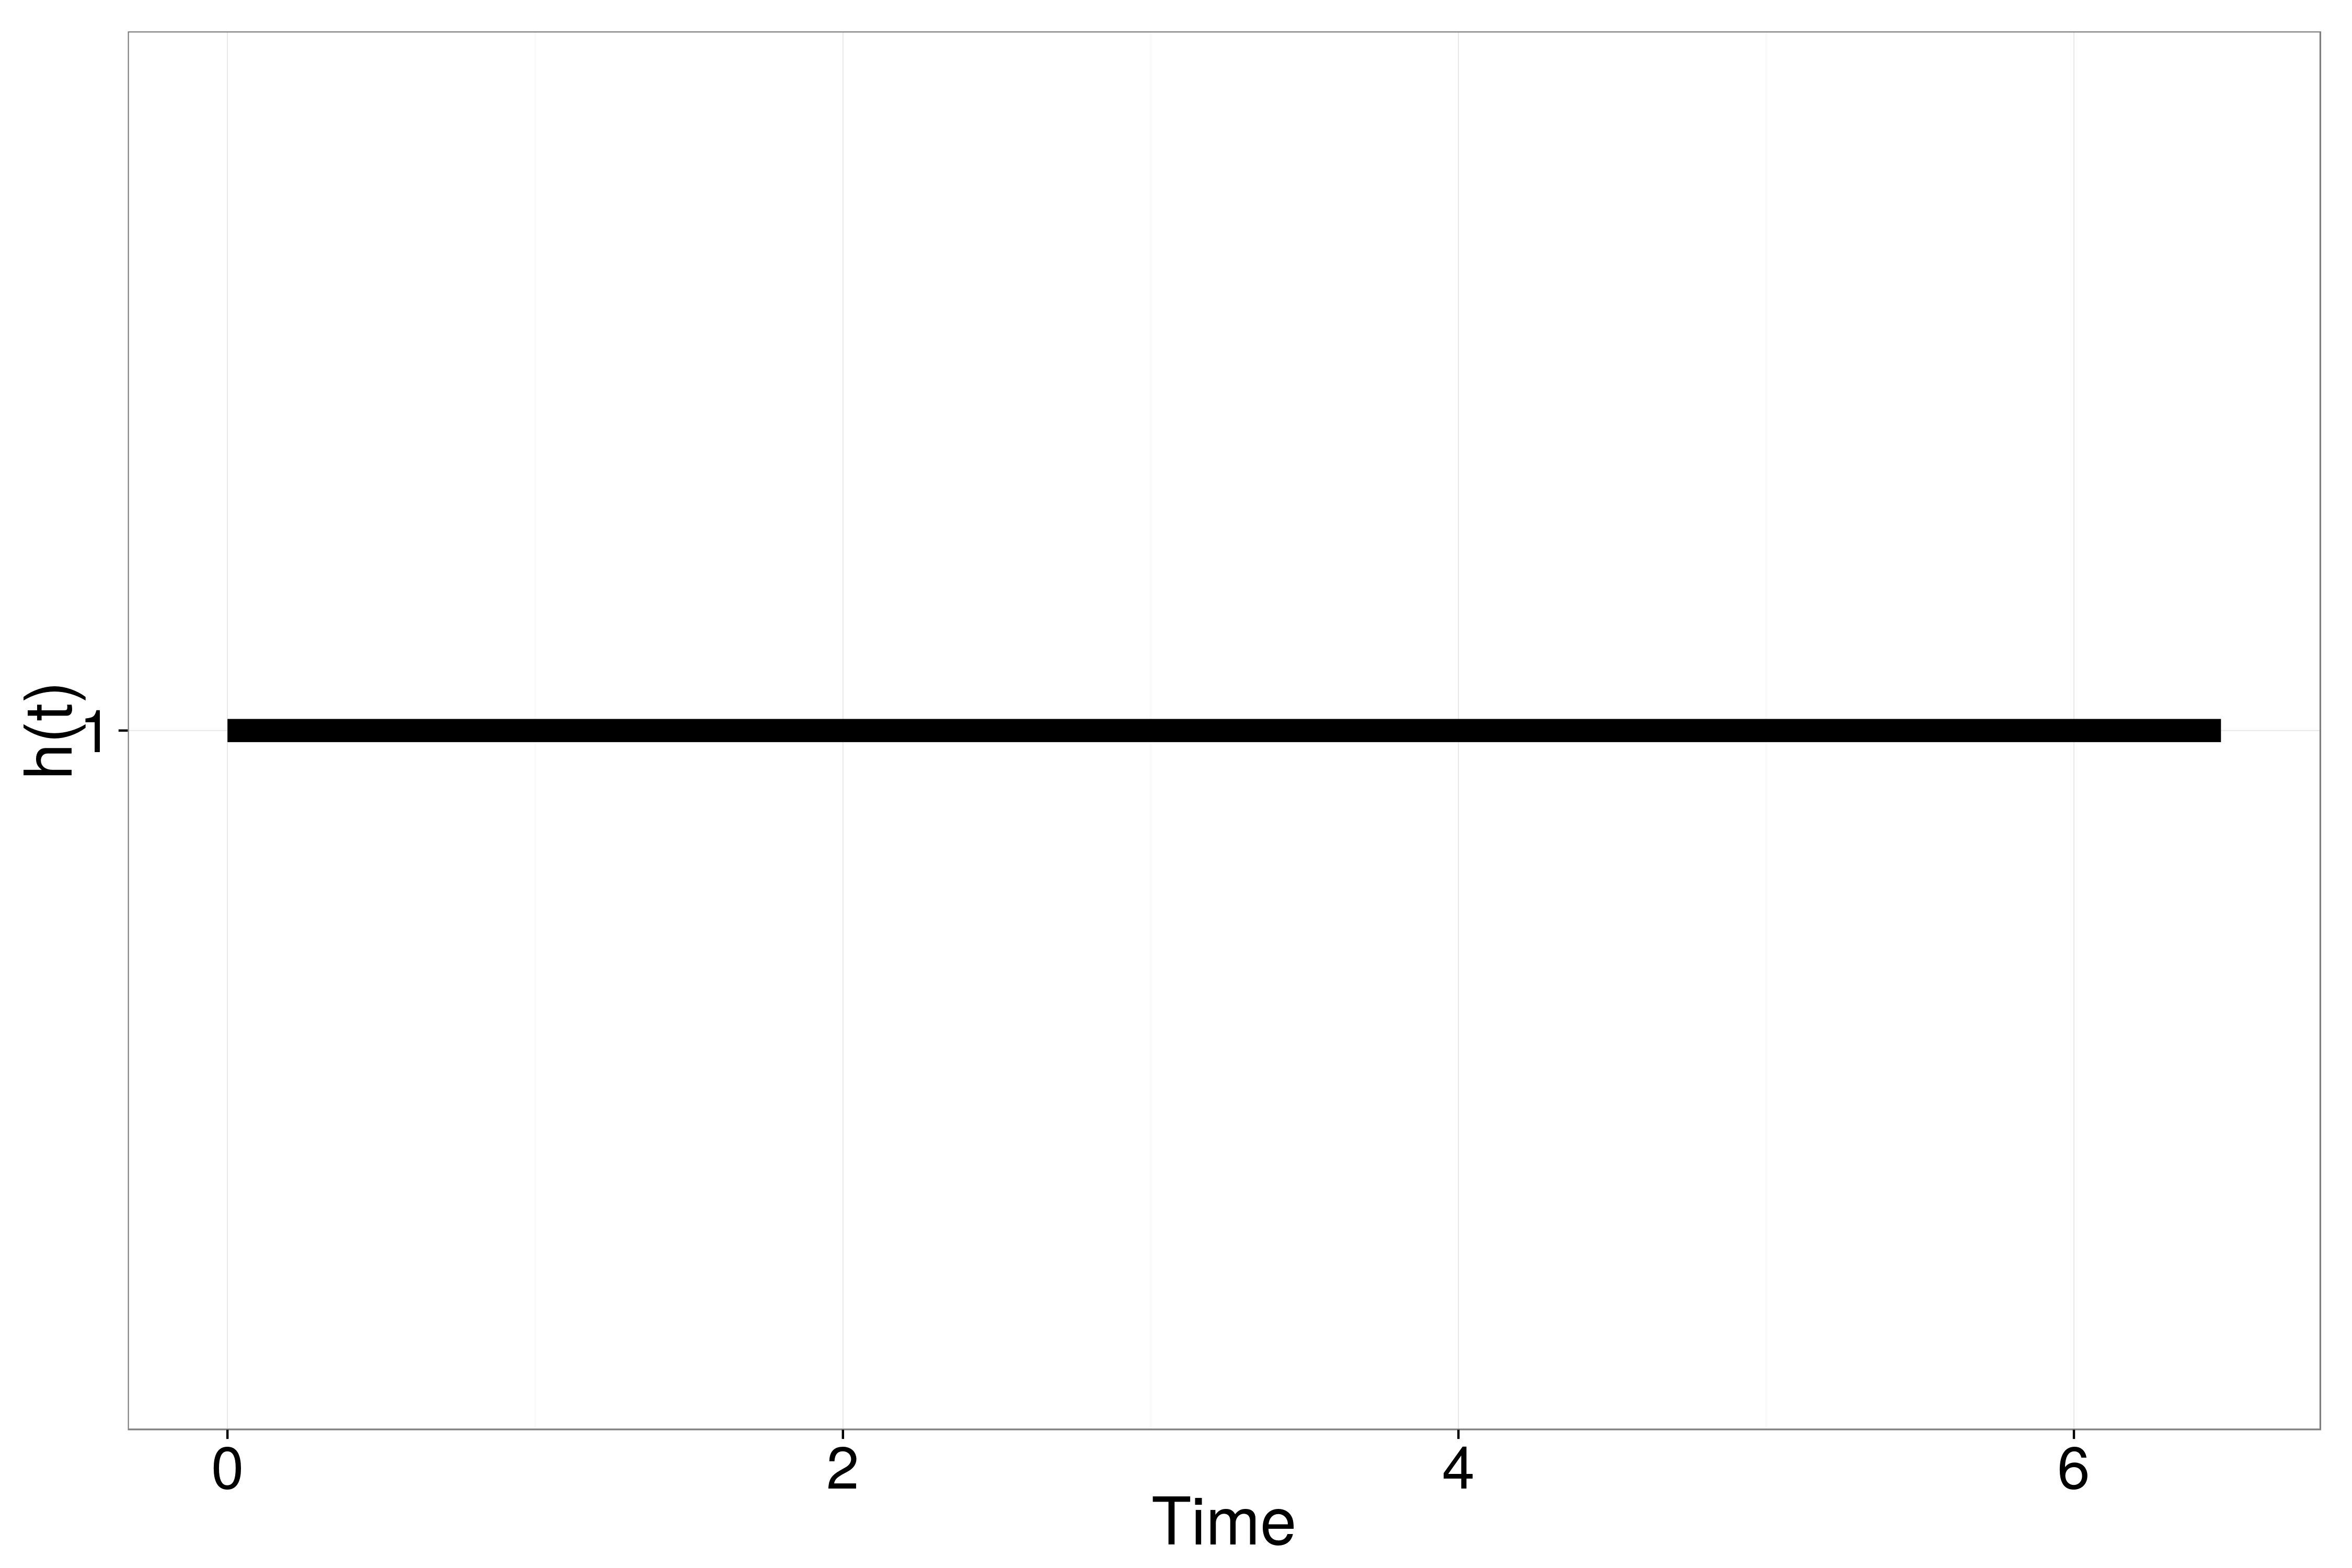
\includegraphics[height = 0.5\textheight, width = 0.4\textwidth, keepaspectratio = true]{figure/haz_exp}
  \end{center}
\end{frame}

\begin{frame}
  \frametitle{Survival analysis}

  \begin{center}
    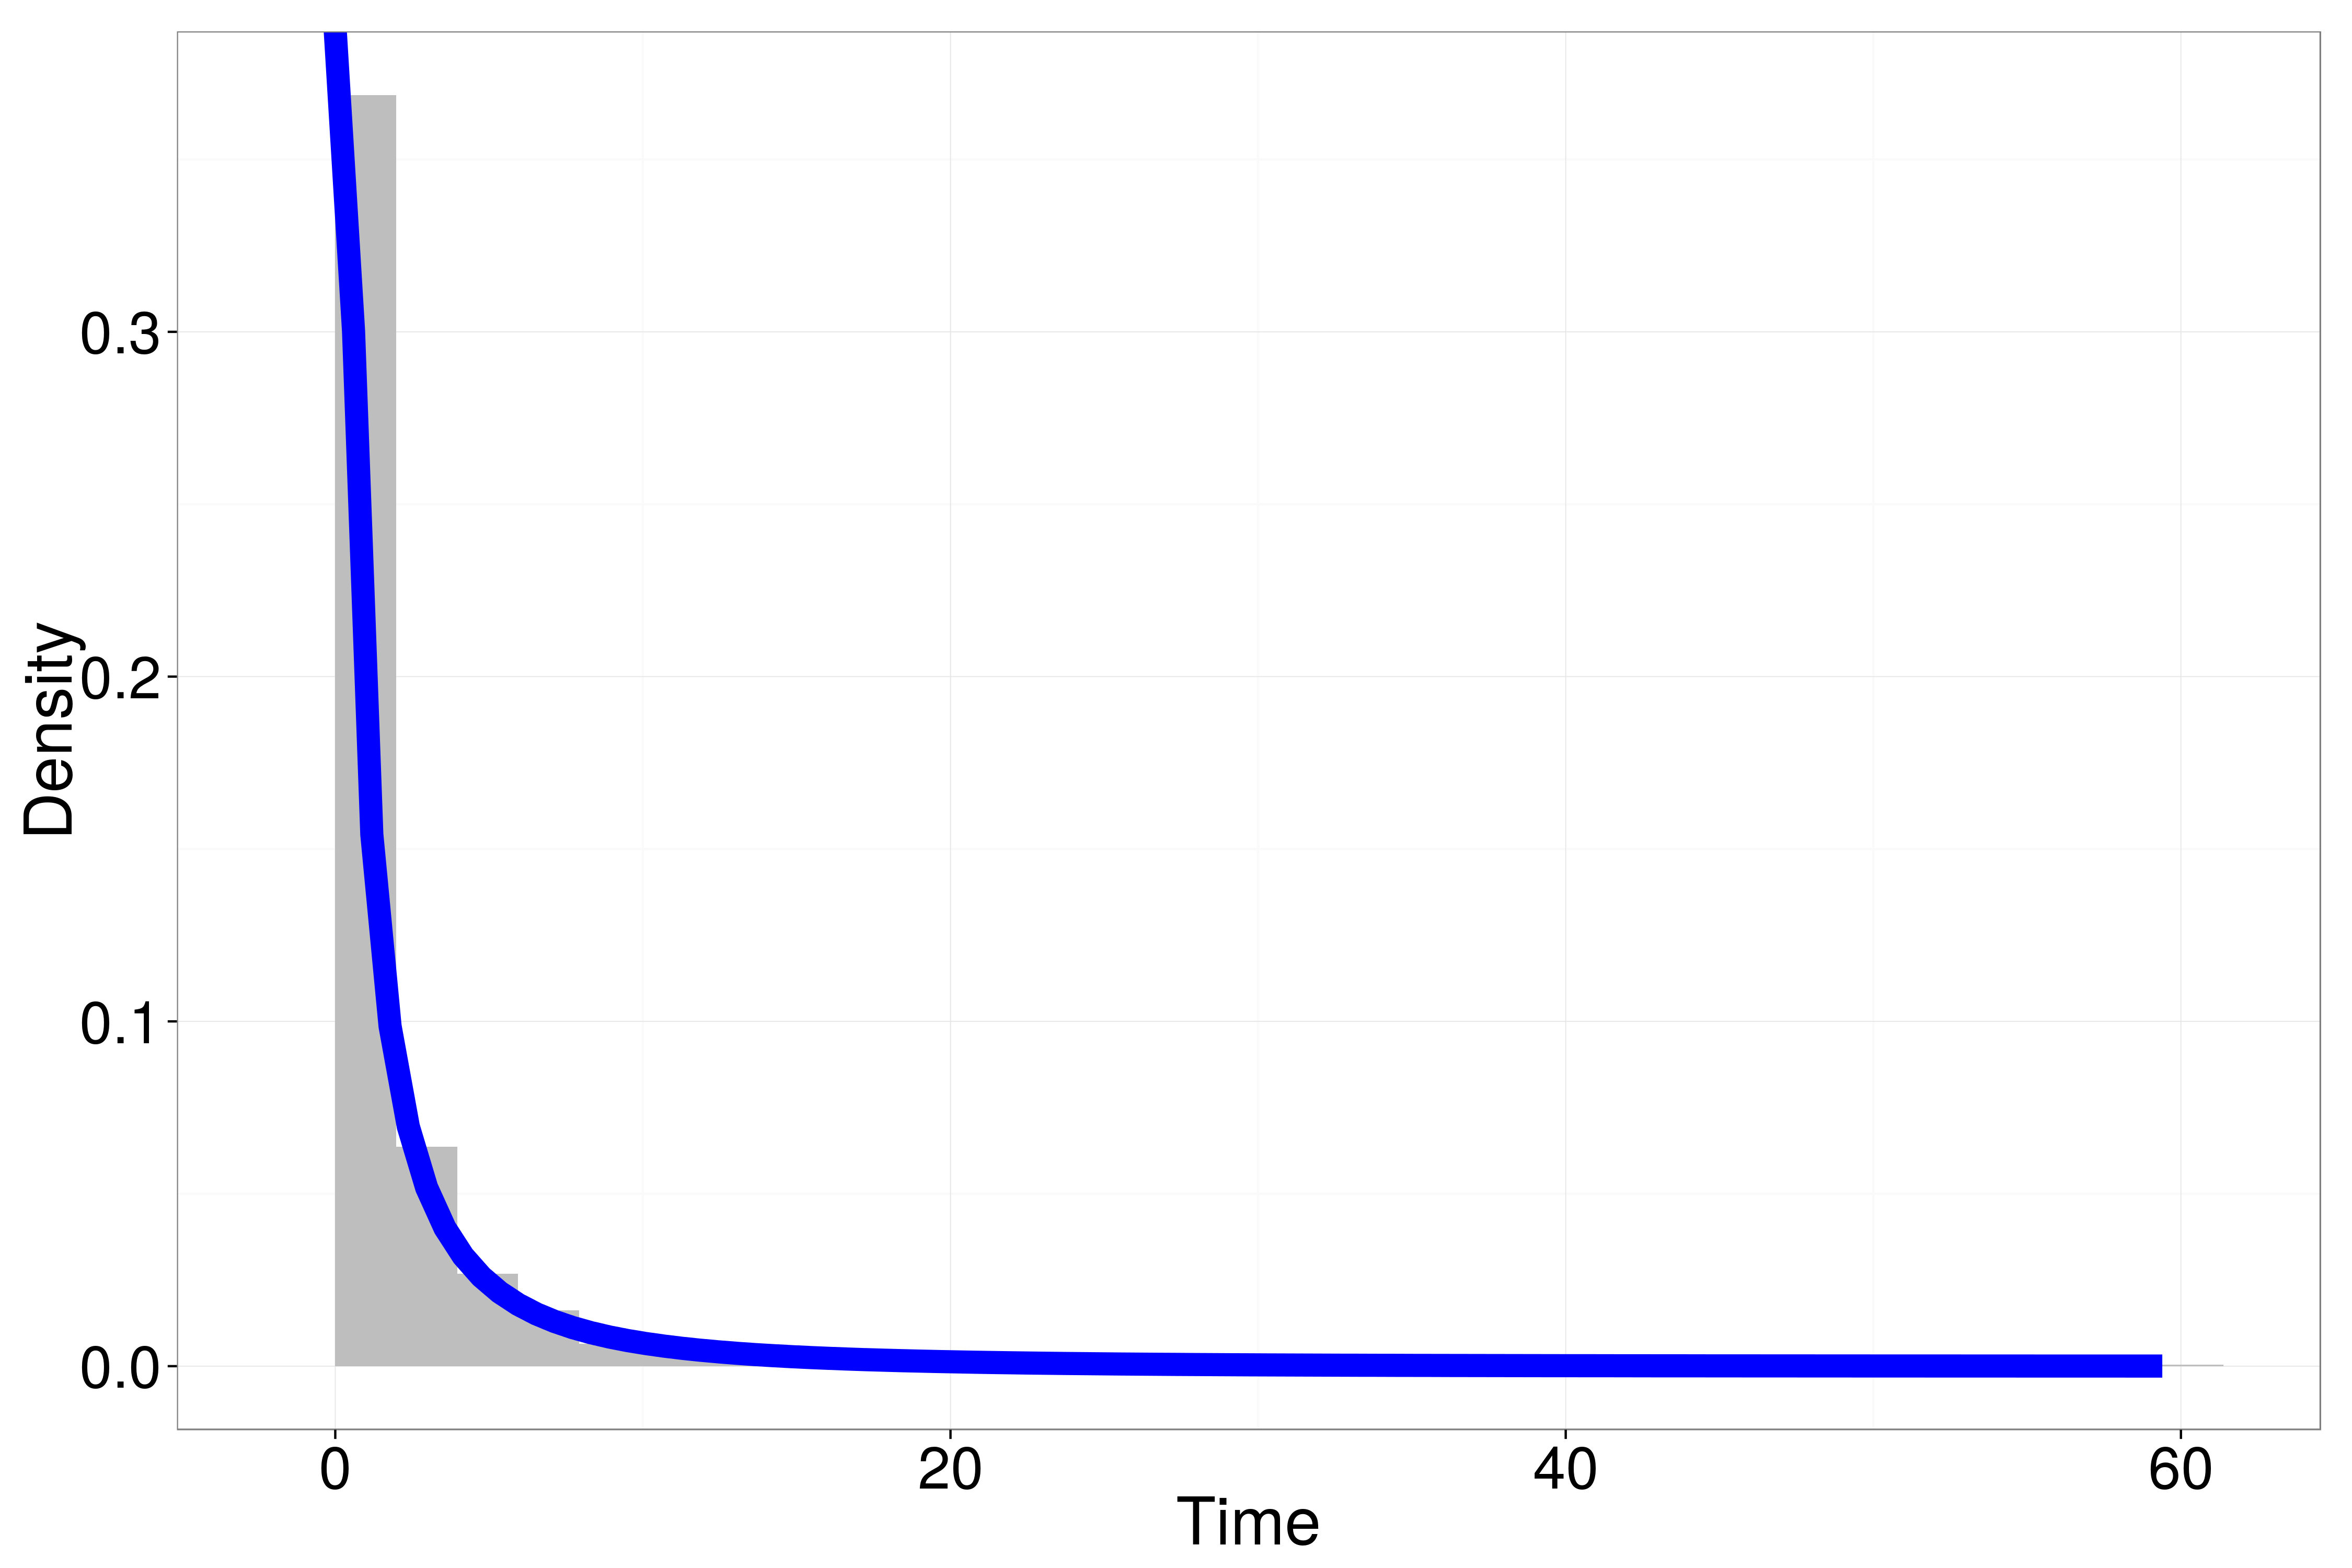
\includegraphics[height = 0.5\textheight, width = \textwidth, keepaspectratio = true]{figure/dur_dec}

    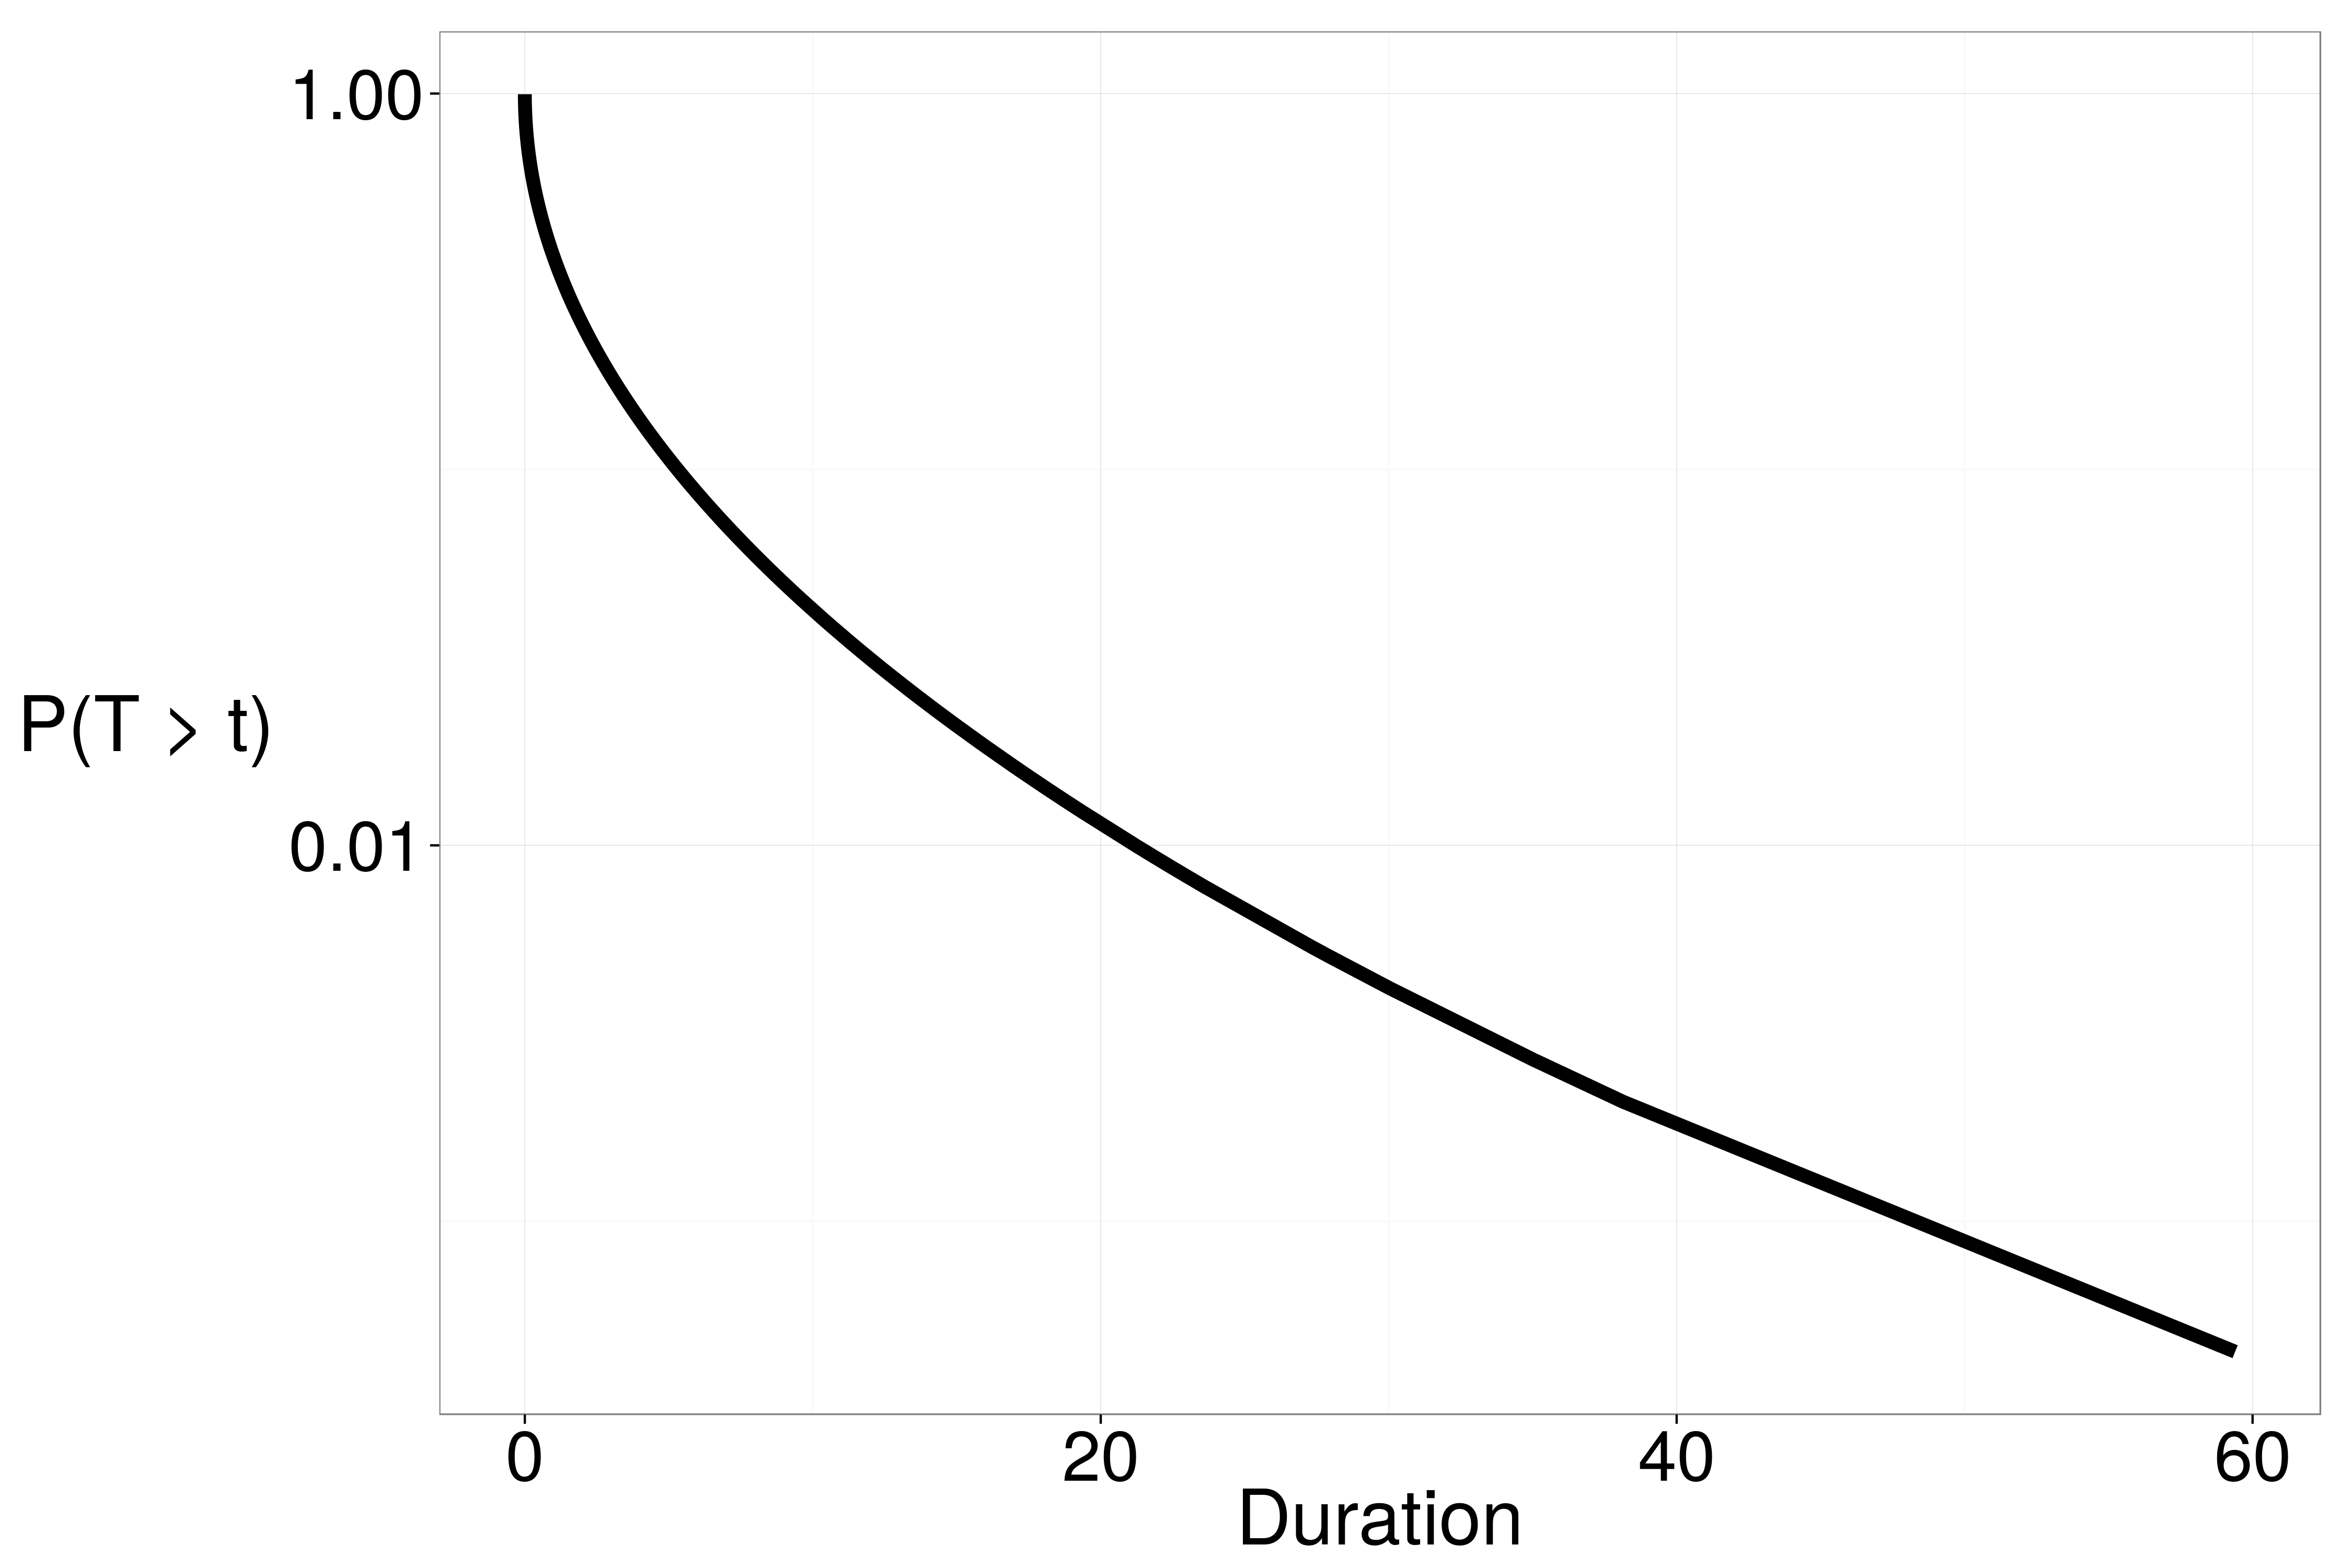
\includegraphics[height = 0.5\textheight, width = 0.4\textwidth, keepaspectratio = true]{figure/sur_dec}
    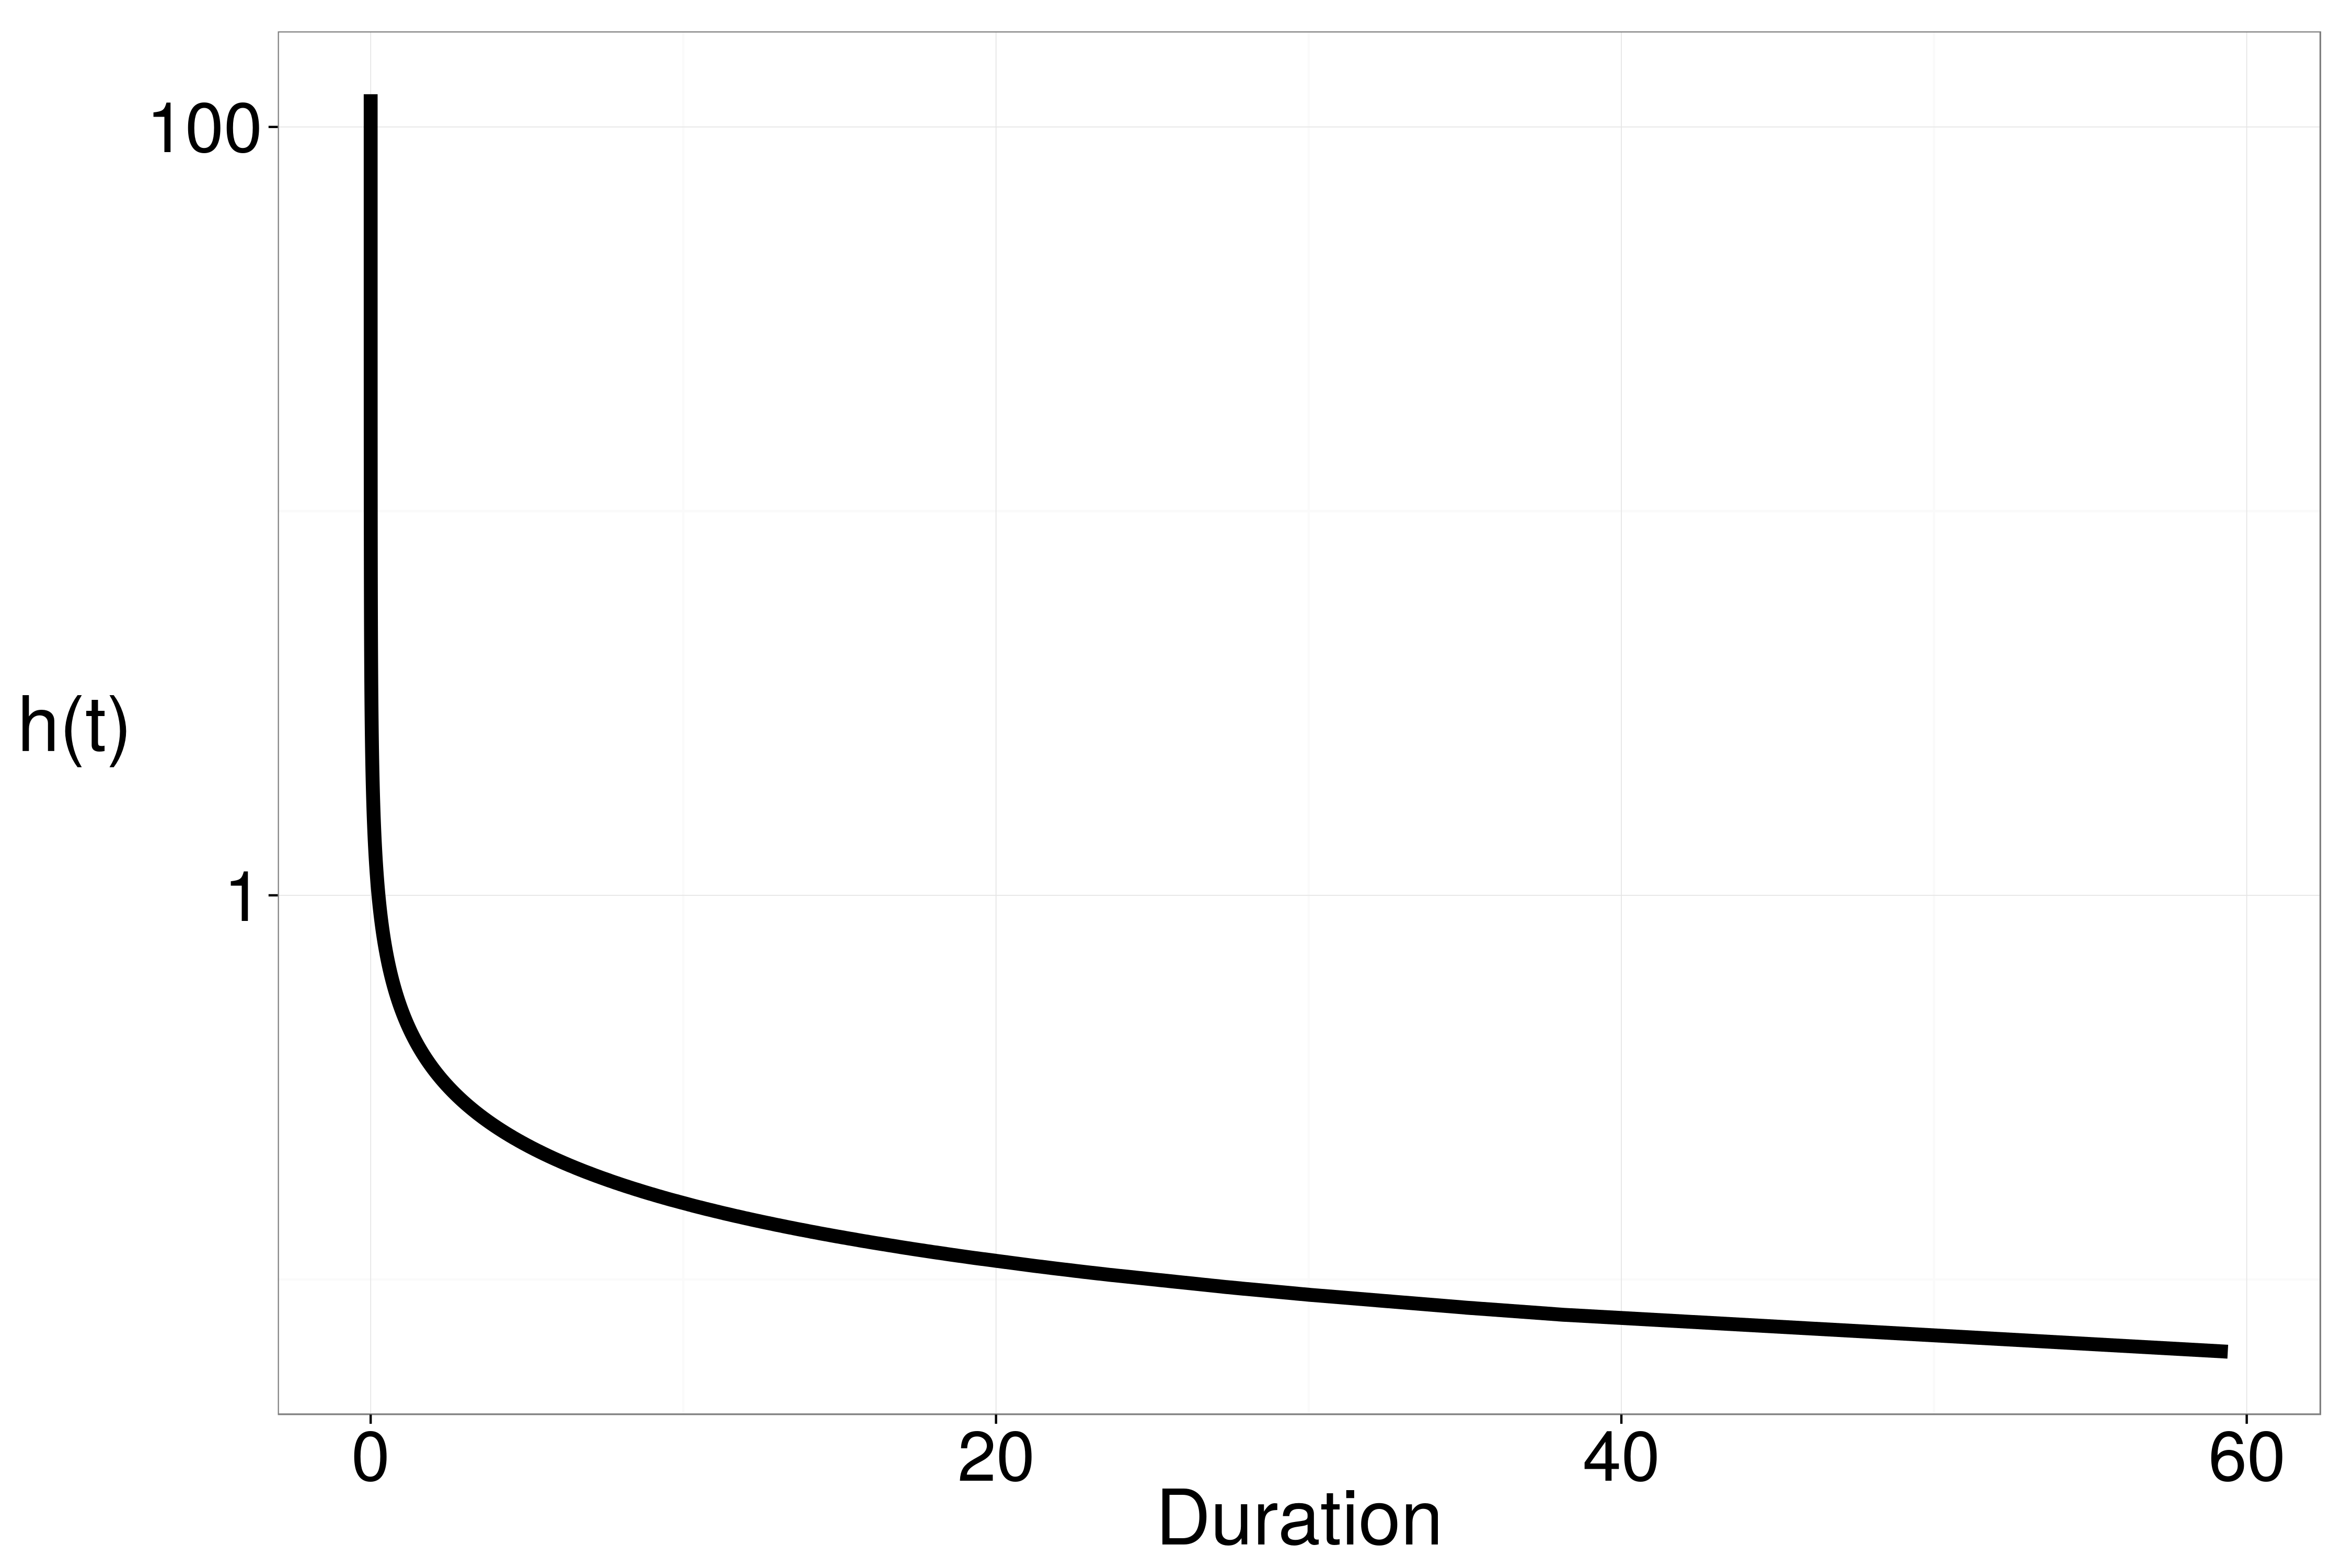
\includegraphics[height = 0.5\textheight, width = 0.4\textwidth, keepaspectratio = true]{figure/haz_dec}
  \end{center}
\end{frame}

\begin{frame}
  \frametitle{Survival analysis}

  \begin{center}
    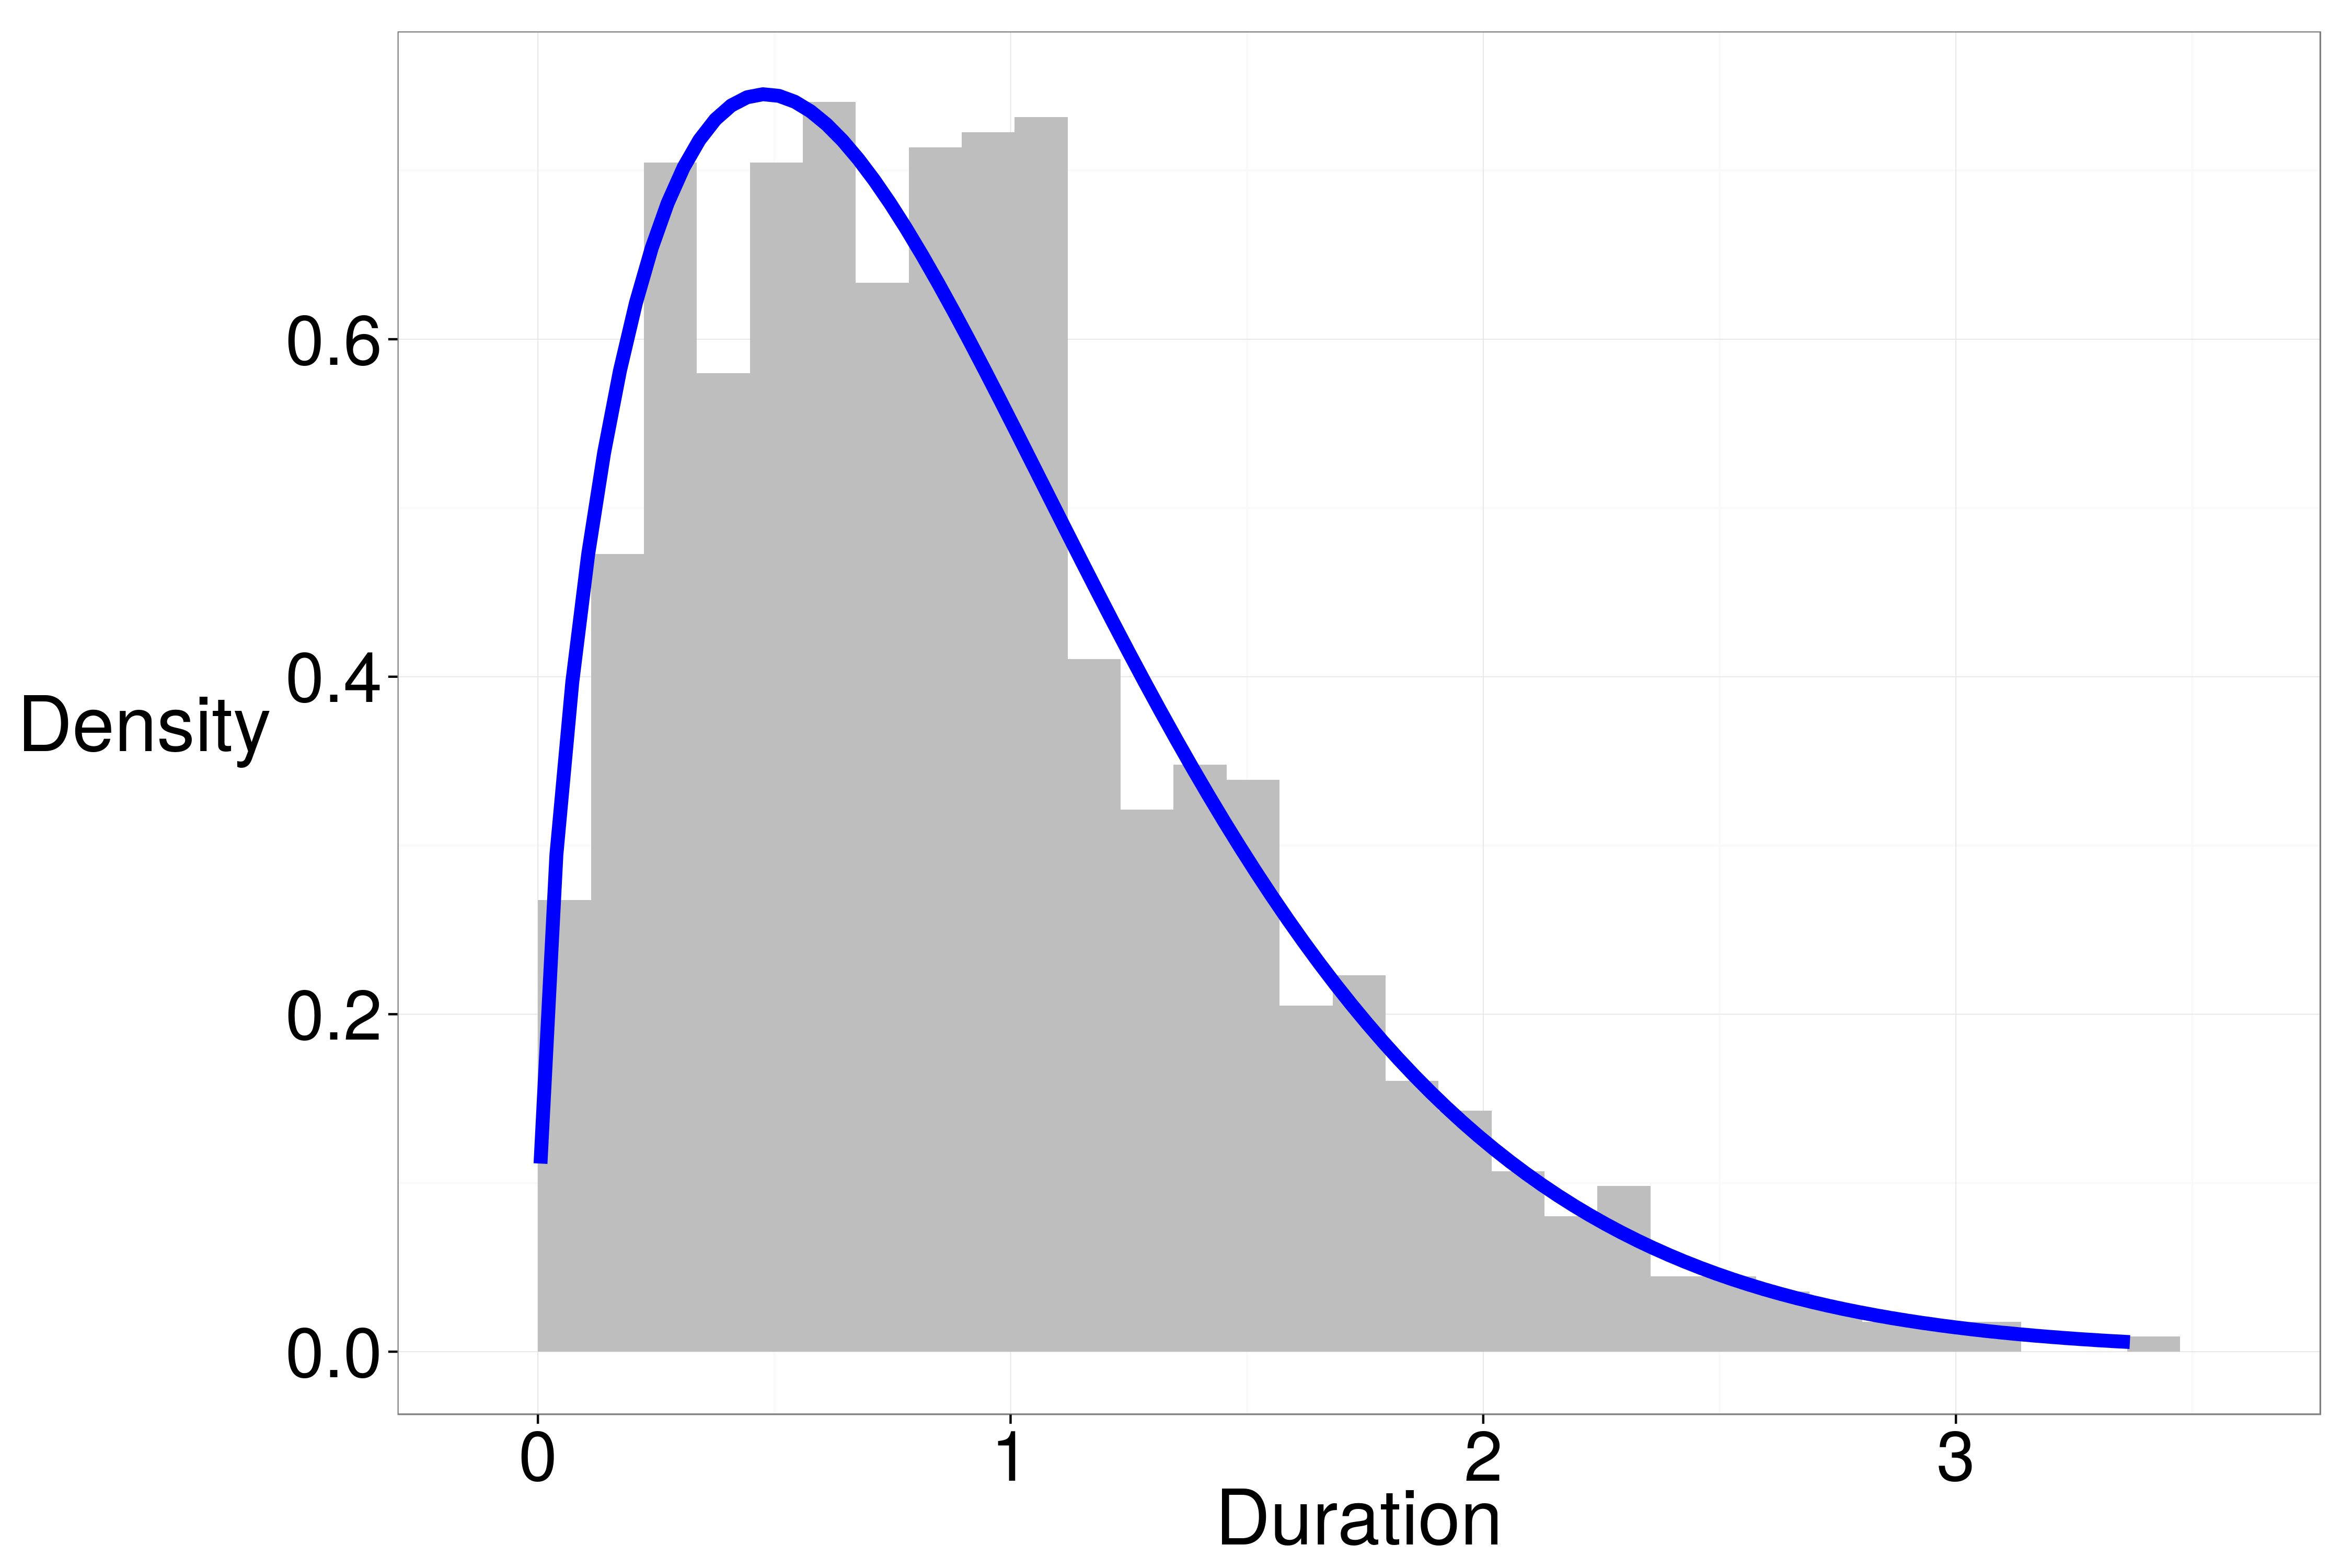
\includegraphics[height = 0.5\textheight, width = \textwidth, keepaspectratio = true]{figure/dur_acc}

    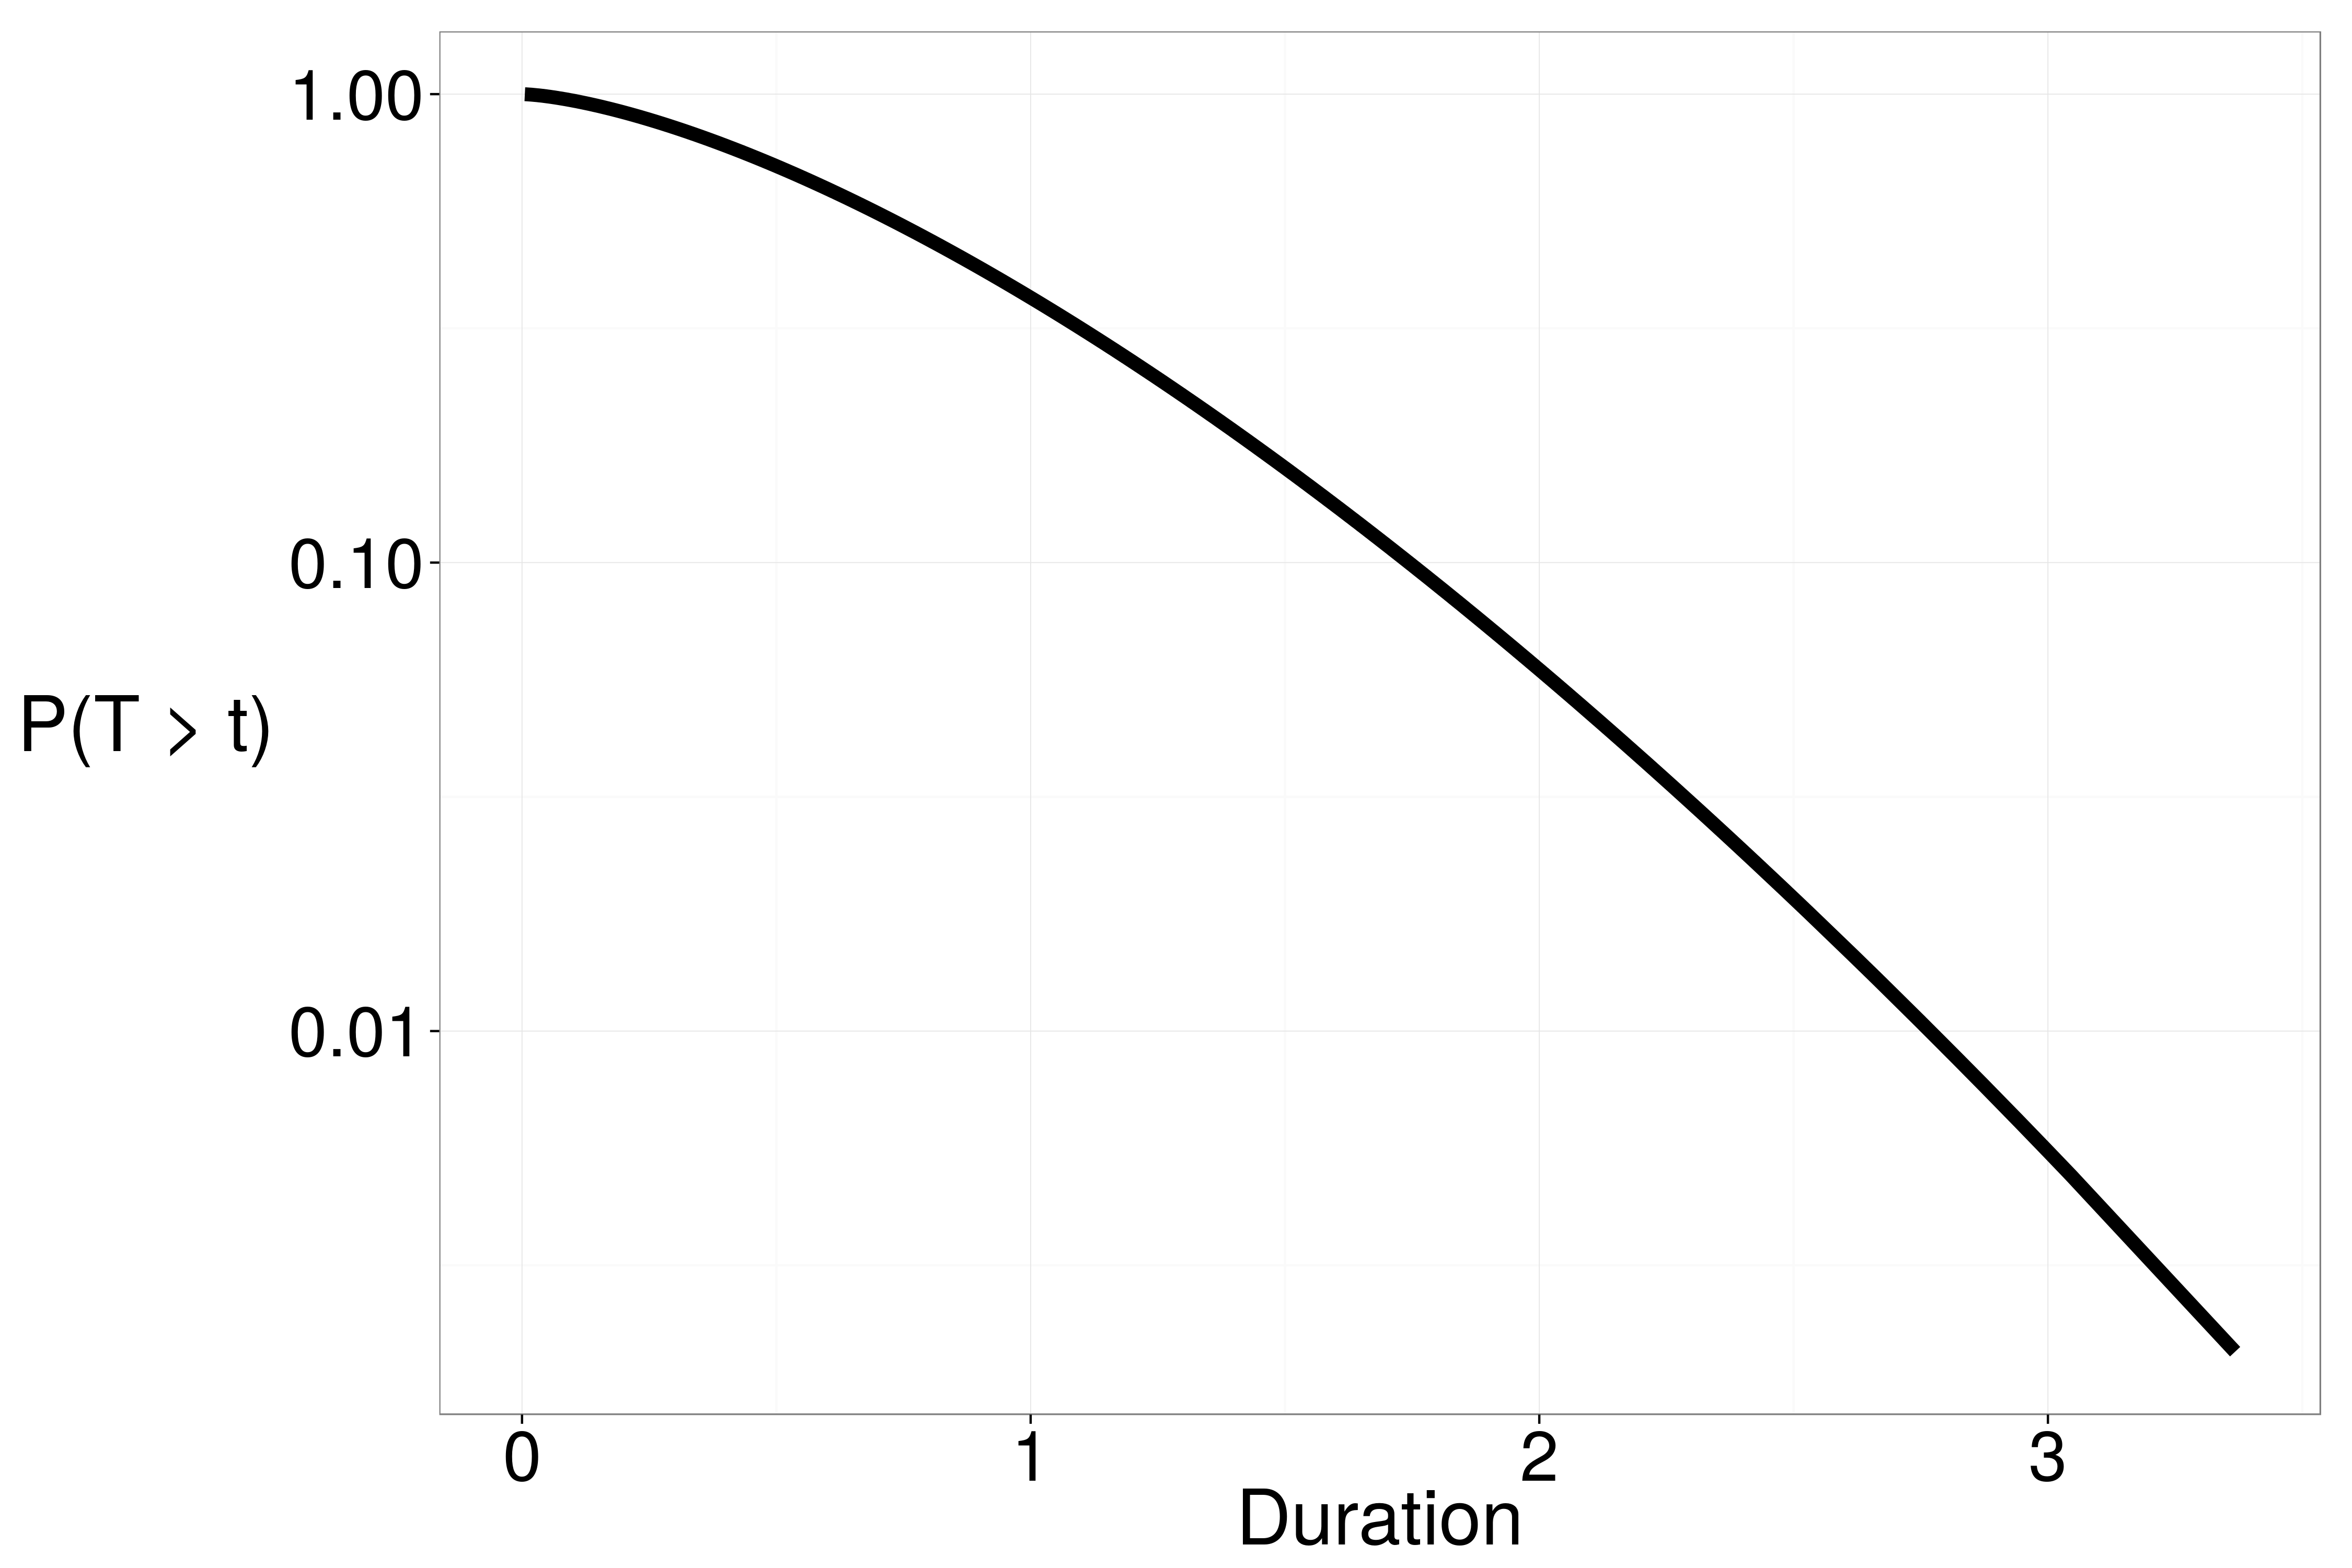
\includegraphics[height = 0.5\textheight, width = 0.4\textwidth, keepaspectratio = true]{figure/sur_acc}
    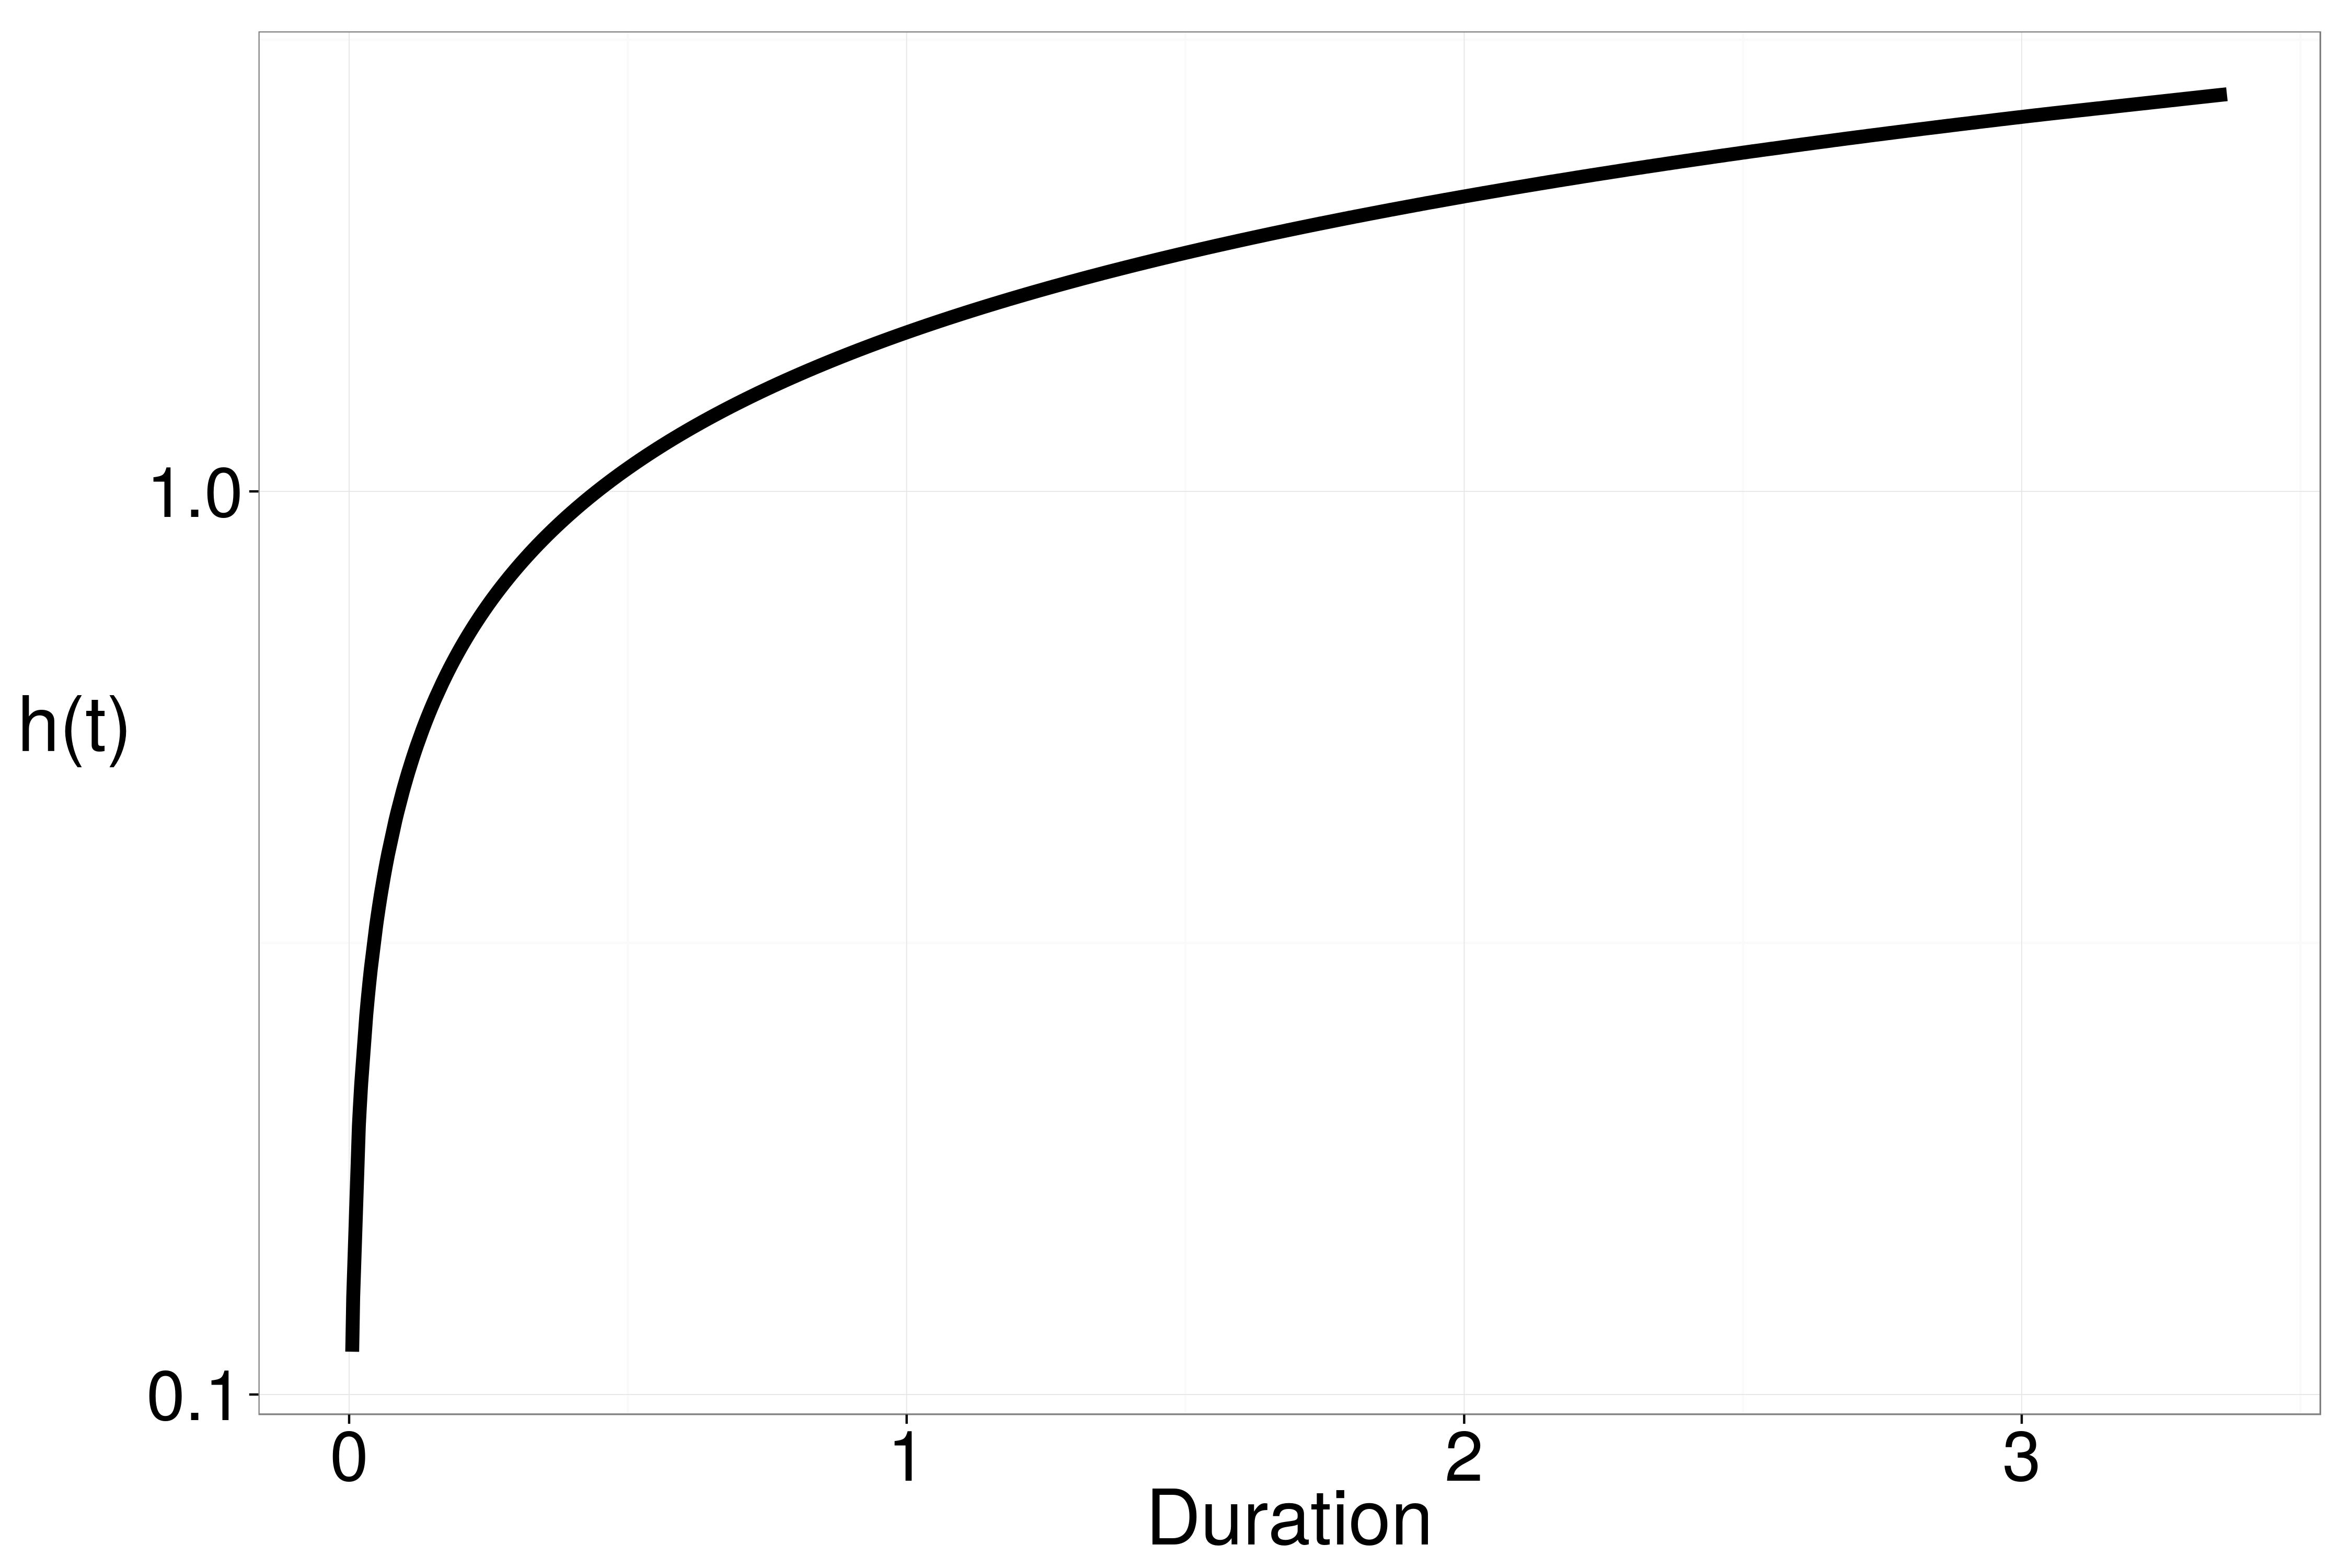
\includegraphics[height = 0.5\textheight, width = 0.4\textwidth, keepaspectratio = true]{figure/haz_acc}
  \end{center}
\end{frame}


\begin{frame}  % make this is krushke like diagram
  \frametitle{Bayesian model structure}
  \begin{center}
    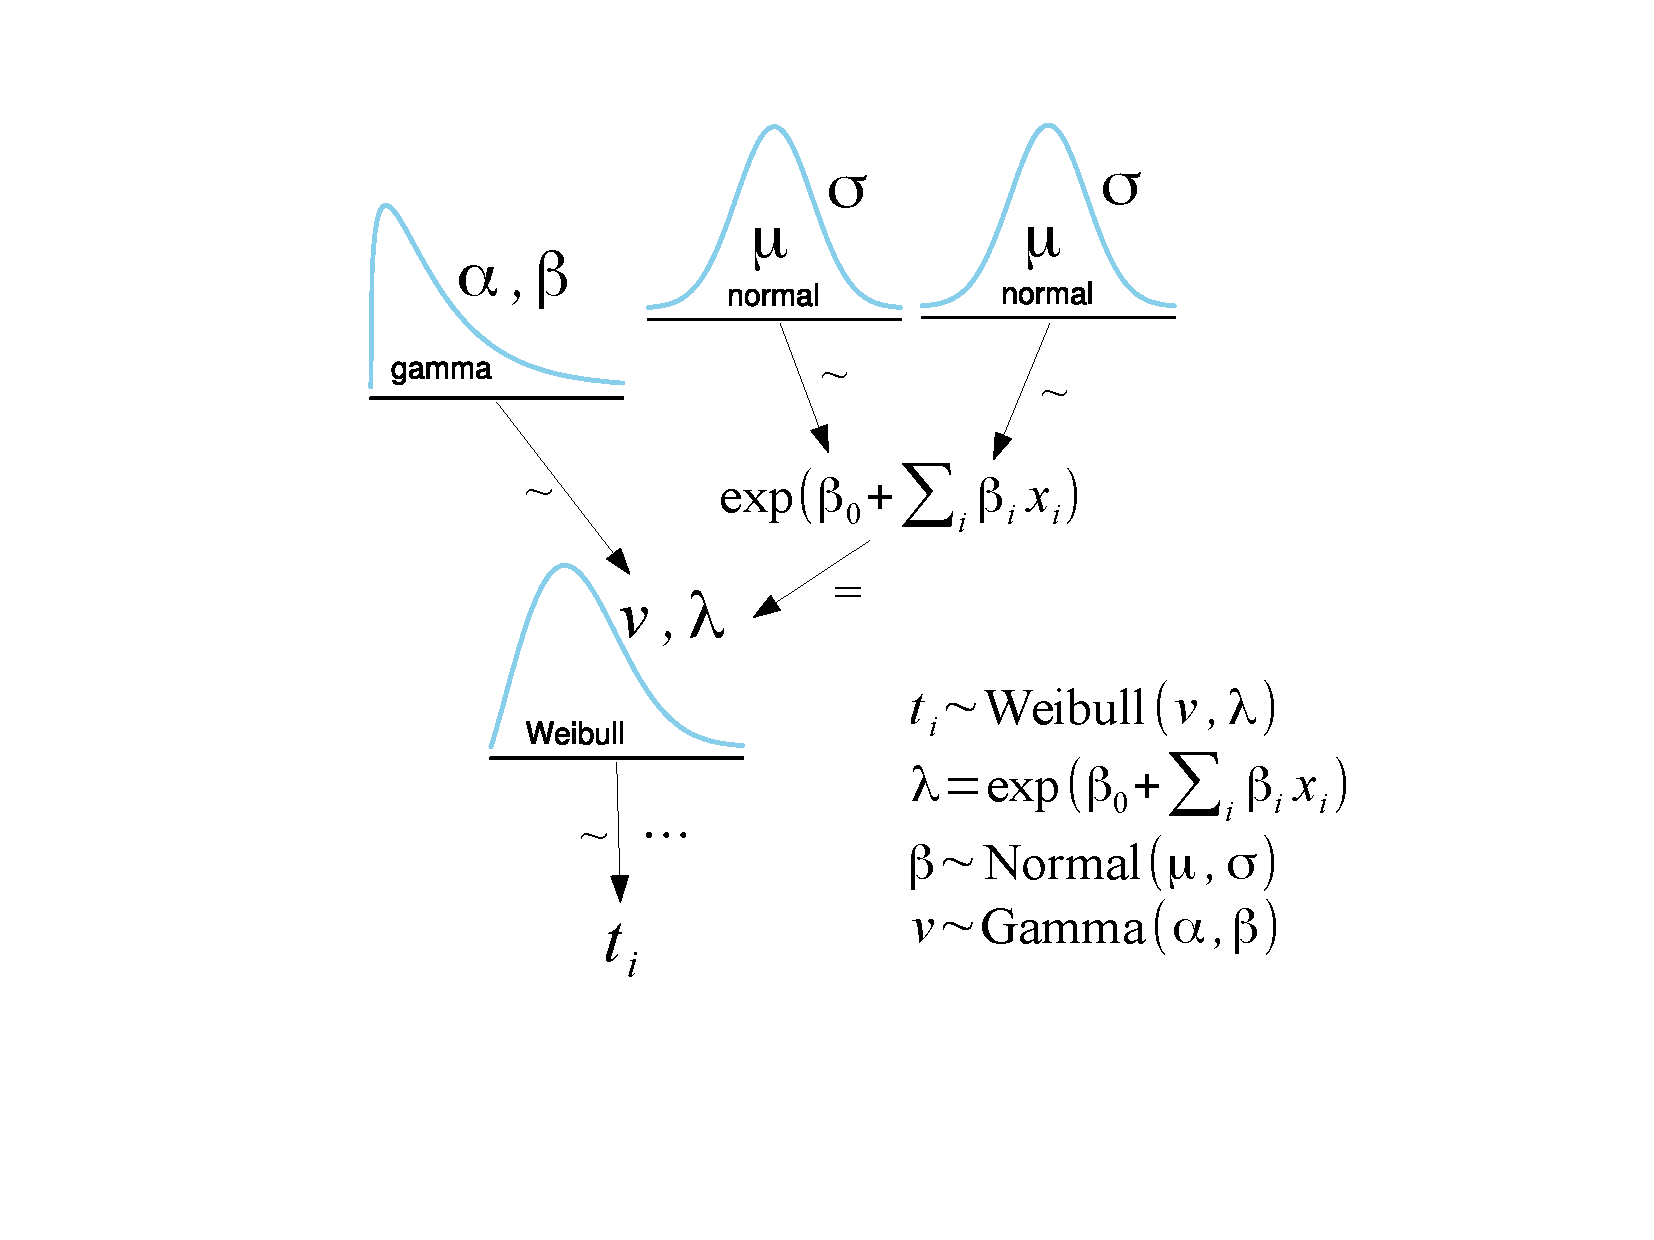
\includegraphics[height = 0.8\textheight, width = \textwidth, keepaspectratio = true]{figure/surv_mod}
  \end{center}
\end{frame}


\begin{frame}  % effect size
  \frametitle{Scale parameter}
  % faceted histograms, one for each beta
  % plot as exp(beta)? to show effect on scale parameter
\end{frame}

\begin{frame}  
  \frametitle{Shape parameter}
  % plot as log(shape) so it is ``centered'' around 0 and easier to interpret
\end{frame}


\begin{frame}  % S(t) and h(t)
  \frametitle{Survival distributions}
\end{frame}


\begin{frame}  % what do we know so far? which parameters to matter most how does that relate to the record?
  \frametitle{Current conclusions}
\end{frame}


\begin{frame}  % improve the data (NZ, etc) and model
  \frametitle{Improvements}
  \begin{columns}
    \begin{column}{0.5\textwidth}
      \begin{itemize}
        \item Data
          \begin{itemize}
            \item New Zealand (FRED)
            \item Improved paleoenvironment reconstructions
            \item affixing strategy information
          \end{itemize}
      \end{itemize}
    \end{column}
    \begin{column}{0.5\textwidth}
      \begin{itemize}
        \item Model
          \begin{itemize}
            \item substrate, habitat as distributions (fully hierarchical model)
            \item sampling rate as predictor
          \end{itemize}
      \end{itemize}
    \end{column}
  \end{columns}
\end{frame}


\begin{frame}
  \frametitle{Acknowledgements}
  \begin{columns}
    \begin{column}{0.4\textwidth}
      \begin{itemize}
        \item Advising
          \begin{itemize}
            \item Kenneth D. Angielczyk, Michael J. Foote, P. David Polly, Richard H. Ree
          \end{itemize}

        \item Discussion 
          \begin{itemize}
            \item David Bapst, Megan Boatright, Ben Frable, Marites Villarosa Garcia, Kathleen Ritterbush, Darcy Ross, Liz Sander, Carl Simpson
          \end{itemize}
      \end{itemize}
    \end{column}
    \begin{column}{0.6\textwidth}
      
\includegraphics[height = 0.3\textheight, keepaspectratio = true]{figure/chicago} 
      
\includegraphics[width = 0.4\textwidth, keepaspectratio = true]{figure/field}

      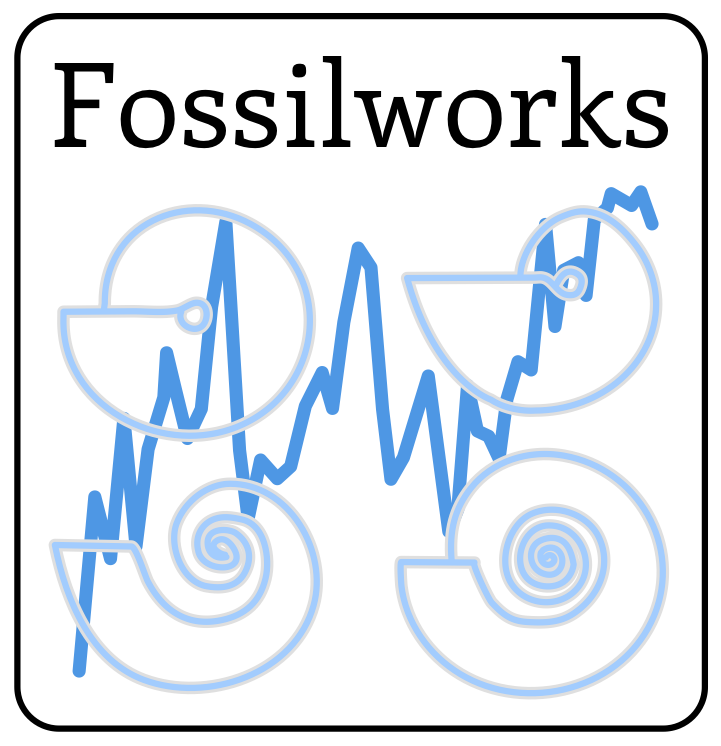
\includegraphics[height = 0.3\textheight, width = 0.5\textwidth, keepaspectratio = true]{figure/fossilworks}
      
\includegraphics[width = 0.5\textwidth, keepaspectratio = true]{figure/paleodb}

    \end{column}
  \end{columns}
\end{frame}

\begin{frame}  % posterior predictive checking, sensitivity analysis
  \frametitle{Model checking}
  % mean survival time
  % median survival time
  % variance?
\end{frame}  % is this actually necessary for what i want to show?

\begin{frame}
  \frametitle{Model formulation}
  \begin{align*}
    p(\lambda, k \mid y) &\propto p(y \mid \lambda, k) p(\lambda, k) \\
    p(y \mid \lambda, k) &= \prod_{i: I_i = 1} Weibull(y \mid \lambda, k) \prod_{i: I_{i} = 0} cCDF_{Weibull}(y, \lambda, k) \\
    \lambda &= \exp(\beta \mathbf{X})\\
    \beta &\sim \mathcal{N}(0, 100) \\
    k &\sim Gamma(1, 1) \\
  \end{align*}
\end{frame}
\end{document}
